\documentclass[openany,a4paper,10pt]{book}

% Define the version number here
% This is automatically incremented when using the commitAll.sh script.
\newcommand{\version}{Version 2.026}

\usepackage[utf8]{inputenc}
\usepackage{amsmath,amssymb, amscd,amsbsy, amsthm, enumerate}
\usepackage{graphicx}
\usepackage{geometry}
\usepackage{titlesec}
\usepackage{lipsum}
\usepackage{wrapfig}
\usepackage{multicol}
\usepackage{listings}
\usepackage{xcolor}
\usepackage{appendix}

%used for custom page headers and page numbering
\usepackage{fancyhdr}

\usepackage{hyperref}

%enables indexing
\usepackage{makeidx}


\usepackage[T1]{fontenc}

\usepackage{tabularx}
%\renewcommand{\chaptername}{}

%\titleformat{\chapter}[display]{\normalfont\bfseries}{}{0pt}{\huge}

\geometry{margin=1in}

\setlength{\parindent}{25pt}

\renewcommand\bibname{References}

\renewcommand{\headrulewidth}{0pt}
%\setcounter{chapter}{-1} %starts the chapter labels at 0 instead of 1

\definecolor{backcolour}{rgb}{0.95,0.95,0.92}
\definecolor{commentcolour}{rgb}{.00,.245,.0}
\definecolor{lightgray}{gray}{0.9}
\lstdefinestyle{sharpc}{language=[Sharp]C, tabsize=3, backgroundcolor=\color{backcolour},breaklines=true, basicstyle=\footnotesize, showstringspaces=false, commentstyle=\color{commentcolour}, keywordstyle=\color{blue}}
\lstset{style=sharpc}


%%% This defines the note environment for you to write your solutions.
\newenvironment{note}
{\let\oldqedsymbol=\qedsymbol
	\renewcommand{\qedsymbol}{$ $}
	\begin{proof}[\bfseries\upshape \color{red}Note]\color{red}}
	{\end{proof}
	\renewcommand{\qedsymbol}{\oldqedsymbol}}

\newcommand{\inlinecode}[1]{\colorbox{lightgray}{\lstinline{#1}}}




%%Different lstlisting formats go here

% Define the custom terminal style
\lstdefinestyle{terminalstyle}{
	language=bash,                   % Set the language to Bash
	basicstyle=\ttfamily\color{white}, % Use a monospaced font and white text
	backgroundcolor=\color{black},   % Background color
	frame=tb,                        % Top and bottom frame lines
	framerule=0.5pt,                 % Frame rule width
	xleftmargin=5pt,                % Left margin
	xrightmargin=0pt,                % Right margin
	rulecolor=\color{black!20},      % Frame color
	showstringspaces=false,          % Don't show spaces in strings
	upquote=true,                    % Use straight quotes
	commentstyle=\color{green},      % Comments are green
	keywordstyle=\color{orange!60},  % Keywords
	numbers=left,                    % Line numbers on the left
	numberstyle=\tiny\color{black!90},   % Line number style
	captionpos=b,                    % Caption position (bottom)
	breaklines=true,                 % Automatically break long lines
	postbreak=\mbox{\textcolor{green}{$\hookrightarrow$}\space}, % Line continuation symbol
}

% Define a bash/shell style.
\lstdefinestyle{shellstyle}{
	language=sh,                    % Set the language to Shell
	basicstyle=\ttfamily,           % Use a monospaced font
	backgroundcolor=\color{gray!10},% Background color
	keywordstyle=\color{blue},      % Keywords are blue
	commentstyle=\color{green!40!black}, % Comments are green
	stringstyle=\color{red},        % Strings are red
	rulecolor=\color{black},        % Frame color
	breakatwhitespace=false,        % Don't break lines at whitespace
	breaklines=true,                % Automatically break long lines
	postbreak=\mbox{\textcolor{red}{$\hookrightarrow$}\space}, % Line continuation symbol
	showstringspaces=false,         % Don't show spaces in strings
	captionpos=b,                   % Caption position (bottom)
	frame=single,                   % Add a frame around listings
	numbers=left,                   % Line numbers on the left
	numberstyle=\tiny\color{gray},  % Line number style
	stepnumber=1,                   % Line number increments
	tabsize=4,                      % Tab size
	xleftmargin=5pt,               % Left margin
	xrightmargin=0pt                % Right margin
}

% Define Python style
\lstdefinestyle{pythonstyle}{
	language=Python,
	basicstyle=\ttfamily\small,
	numbers=left,
	numberstyle=\tiny\color{gray},
	frame=single,
	rulecolor=\color{orange},
	backgroundcolor=\color{orange!05},
	keywordstyle=\color{blue},
	commentstyle=\color{green!40!black},
	stringstyle=\color{red},
	breaklines=true,
	tabsize=4,
	captionpos=b,
	extendedchars=true,
	inputencoding=utf8,
	showspaces=false,
	showstringspaces=false,
	xleftmargin=5pt,               % Left margin
	xrightmargin=0pt                % Right margin
}


% Define C++ style
\lstdefinestyle{cppstyle}{
	language=C++,
	basicstyle=\ttfamily\small,
	numbers=left,
	numberstyle=\tiny\color{gray},
	frame=single,
	rulecolor=\color{black!30},
	backgroundcolor=\color{gray!05},% Background color
	keywordstyle=\color{blue},
	commentstyle=\color{green!40!black},
	stringstyle=\color{red},
	breaklines=true,
	tabsize=4,
	captionpos=b,
	extendedchars=true,
	inputencoding=utf8,
	showspaces=false,
	showstringspaces=false,
	xleftmargin=5pt,               % Left margin
	xrightmargin=0pt                % Right margin
}

% Define dark green color
\definecolor{darkgreen}{RGB}{0,100,0}

% Define Makefile style
\lstdefinestyle{makestyle}{
	language=make,
	basicstyle=\ttfamily\small,
	numbers=left,
	numberstyle=\tiny\color{gray},
	frame=single,
	backgroundcolor=\color{darkgreen!05},
	rulecolor=\color{darkgreen},
	keywordstyle=\color{blue},
	commentstyle=\color{green!40!black},
	stringstyle=\color{red},
	breaklines=true,
	tabsize=4,
	captionpos=b,
	extendedchars=true,
	inputencoding=utf8,
	showspaces=false,
	showstringspaces=false,
	xleftmargin=5pt,               % Left margin
	xrightmargin=0pt                % Right margin
}

% Define Git style
\lstdefinestyle{gitstyle}{
	language=bash, % Assuming Git commands are written in a bash-like language
	basicstyle=\ttfamily\small,
	numbers=left,
	numberstyle=\tiny\color{gray},
	frame=single,
	backgroundcolor=\color{blue!05},
	rulecolor=\color{blue},
	keywordstyle=\color{blue},
	commentstyle=\color{green!40!black},
	stringstyle=\color{red},
	breaklines=true,
	tabsize=4,
	captionpos=b,
	extendedchars=true,
	inputencoding=utf8,
	showspaces=false,
	showstringspaces=false,
	xleftmargin=5pt,               % Left margin
	xrightmargin=0pt                % Right margin
}

% Define C# style
\lstdefinestyle{csharpstyle}{
	language=[Sharp]C,
	basicstyle=\ttfamily\small,
	numbers=left,
	numberstyle=\tiny\color{gray},
	frame=single,
	rulecolor=\color{purple},
	backgroundcolor=\color{purple!05},
	keywordstyle=\color{blue},
	commentstyle=\color{green!40!black},
	stringstyle=\color{red},
	breaklines=true,
	tabsize=4,
	captionpos=b,
	extendedchars=true,
	inputencoding=utf8,
	showspaces=false,
	showstringspaces=false,
	xleftmargin=5pt,               % Left margin
	xrightmargin=0pt                % Right margin
}

% Define Java style
\lstdefinestyle{javastyle}{
	language=Java,
	basicstyle=\ttfamily,
	keywordstyle=\color{blue},
	rulecolor=\color{red!80},
	backgroundcolor=\color{red!05},
	commentstyle=\color{green!70!black},
	stringstyle=\color{red},
	numbers=left,
	numberstyle=\tiny\color{gray},
	stepnumber=1,
	breaklines=true,
	breakatwhitespace=false,
	tabsize=4,
	frame=single,
	showspaces=false,
	showstringspaces=false,
	xleftmargin=5pt,               % Left margin
	xrightmargin=0pt                % Right margin
}

% Define JavaScript language settings
\lstdefinelanguage{JavaScript}{
	keywords={typeof, new, true, false, catch, function, return, null, catch, switch, var, if, in, while, do, else, case, break, default},
	keywordstyle=\color{blue}\bfseries,
	ndkeywords={class, export, boolean, throw, implements, import, this},
	ndkeywordstyle=\color{darkgray}\bfseries,
	identifierstyle=\color{black},
	sensitive=false,
	comment=[l]{//},
	morecomment=[s]{/*}{*/},
	commentstyle=\color{purple}\ttfamily,
	stringstyle=\color{red}\ttfamily,
	morestring=[b]',
	morestring=[b]",
}

% Define JavaScript style
\lstdefinestyle{jsstyle}{
	language=JavaScript,
	basicstyle=\ttfamily,
	rulecolor=\color{red!80},
	backgroundcolor=\color{red!05},
	keywordstyle=\color{blue},
	commentstyle=\color{green!70!black},
	stringstyle=\color{red},
	numbers=left,
	numberstyle=\tiny\color{gray},
	stepnumber=1,
	breaklines=true,
	breakatwhitespace=false,
	tabsize=4,
	frame=single,
	showspaces=false,
	showstringspaces=false,
	xleftmargin=5pt,               % Left margin
	xrightmargin=0pt                % Right margin
}

% Define HTML style
\lstdefinestyle{htmlstyle}{
	language=HTML,
	basicstyle=\ttfamily\small,
	numbers=left,
	numberstyle=\tiny\color{gray},
	frame=single,
	rulecolor=\color{black},
	backgroundcolor=\color{yellow!05},
	keywordstyle=\color{blue},
	commentstyle=\color{green!40!black},
	stringstyle=\color{red},
	breaklines=true,
	tabsize=4,
	captionpos=b,
	extendedchars=true,
	inputencoding=utf8,
	showspaces=false,
	showstringspaces=false,
	xleftmargin=5pt,               % Left margin
	xrightmargin=0pt                % Right margin
}

% Define CSS style
\lstdefinestyle{cssstyle}{
	language=HTML,
	basicstyle=\ttfamily\small,
	numbers=left,
	numberstyle=\tiny\color{gray},
	frame=single,
	rulecolor=\color{black},
	keywordstyle=\color{blue},
	commentstyle=\color{green!40!black},
	stringstyle=\color{red},
	breaklines=true,
	tabsize=4,
	captionpos=b,
	extendedchars=true,
	inputencoding=utf8,
	showspaces=false,
	showstringspaces=false,
	xleftmargin=5pt,               % Left margin
	xrightmargin=0pt                % Right margin
}

% Define LaTeX style
\lstdefinestyle{latexstyle}{
	language=TeX,
	basicstyle=\ttfamily\small,
	numbers=left,
	numberstyle=\tiny\color{gray},
	frame=single,
	rulecolor=\color{brown},
	backgroundcolor=\color{brown!05},
	keywordstyle=\color{blue},
	commentstyle=\color{green!40!black},
	stringstyle=\color{red},
	breaklines=true,
	tabsize=4,
	captionpos=b,
	extendedchars=true,
	inputencoding=utf8,
	showspaces=false,
	showstringspaces=false,
	xleftmargin=5pt,               % Left margin
	xrightmargin=0pt                % Right margin
}

% Define PHP style
\lstdefinestyle{phpstyle}{
	language=PHP,
	basicstyle=\ttfamily\small,
	numbers=left,
	numberstyle=\tiny\color{gray},
	frame=single,
	rulecolor=\color{black},
	keywordstyle=\color{blue},
	commentstyle=\color{green!40!black},
	stringstyle=\color{red},
	breaklines=true,
	tabsize=4,
	captionpos=b,
	extendedchars=true,
	inputencoding=utf8,
	showspaces=false,
	showstringspaces=false,
	xleftmargin=5pt,               % Left margin
	xrightmargin=0pt                % Right margin
}

\title{\vspace{0.1cm}  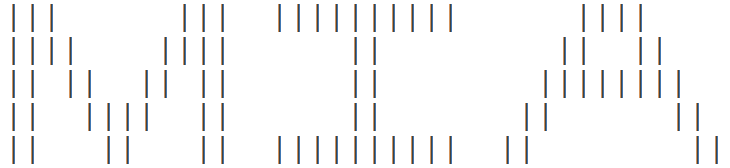
\includegraphics[scale=0.5]{./images/MIA_cropped_Inverted.png} \vspace{.5cm} \\ Multiple Integrated Applications (MIA) \\  Manual \& Programming Documentation}
\author{Developer: Antonius Torode}
\date{Version -- \version \\ Latest update: \today}

\makeindex

\begin{document}

\frontmatter
\maketitle
\pagestyle{empty}
%% copyrightpage
\begingroup
\footnotesize
\parindent 0pt
\parskip \baselineskip
\textcopyright{} 2021 Antonius Torode \\
All rights reserved.

This work may be distributed and/or modified under the conditions of Antonius’ General Purpose License (AGPL).

The Original Maintainer of this work is: Antonius Torode.

The Current Maintainer of this work is: Antonius Torode.

This document is designed for the sole purpose of providing documentation for Multiple Integrated Applications (MIA), a program written for and created for personal use. Throughout this document, ``MIA" will be used as a reference to ``Multiple Integrated Applications." This acronym is solely designed for use in conjunction with the program and was originally created by the creator of this document. MIA is designed to be used for multiple purposes based on the continual addition of functionality. It can be adapted to work in other situations and for alternate purposes.


\begin{center}
\begin{tabular}{ll}
This document is continuously under development. \\
Most Current Revision Date: &  \today 
\end{tabular}
\end{center}

\vfill

Torode, A.\\
\hspace*{1em} MIA Manual. \\
\hspace*{2em} 2021. \\
\hspace*{2em} Includes Source Code and References \\


\endgroup
\clearpage
\tableofcontents
\newpage
\vspace*{\fill}
\begin{center}
	\textit{This page intentionally left blank. \\(Yes, this is a contradiction)}
\end{center}
\vspace*{\fill}

\mainmatter
\pagestyle{fancy}
\fancyhf{}
\fancyhead[RO, LE]{\thepage}


\fancypagestyle{plain}{%
	%\fancyhf{} % clear all header and footer fields
	\fancyhead[RO, LE]{\thepage}
	\renewcommand{\headrulewidth}{0pt}
	\renewcommand{\footrulewidth}{0pt}}

\chapter{Multiple Integrated Applications (MIA)}
\pagestyle{fancy}

\section{Introduction}

MIA is designed to be a collection of scripts, tools, programs, and commands that have been created in the past and may be useful in the future. It's original idea was a place for the original author to combine all of his previous applications and codes into one location that can be compiled cross platform. MIA is written in C++ but will contain codes that were originally designed in C\#, Java, Python, and others. MIA is created for the authors personal use but may be used by others if a need or desire arises under the terms of Antonius’ General Purpose License (AGPL). 

The MIA acronym was created by the original author for the sole purpose of this application. The design of MIA is a terminal prompt that accepts commands. There are no plans to convert MIA into a GUI application as there is currently no need; however, some elements may be programmed in that produce a GUI window for certain uses such as graphs. The MIA manual is designed to be an explanation of what MIA contains as well as a guide of how to utilize the MIA program to it's fullest. 

As MIA is continually under development, this document is also. Due to this, it may fall behind and become slightly outdated as I implement and test new features into MIA. I will attempt to keep this document up to date with all of the features MIA contains but I can only do so if time permits.


















\section{MIA Features}

\subsection{MIA Application Framework}

One of the main features of MIA is the core framework and internal setup. The MIA project's core framework and modular architecture form the backbone of its design, providing a robust, extensible, and developer-friendly ecosystem for building and managing applications. This framework enforces a standardized application life cycle, ensures clear dependency management, and integrates seamlessly with supporting systems such as error handling, configuration, and logging. By leveraging modern C++20 features, the core framework promotes type-safe, maintainable, and scalable application development, making it a cornerstone feature of MIA.

The core framework is built around several interconnected components that collectively enhance modularity and usability:
\begin{itemize}
	\item \textbf{Layered Dependency Structure:} The project is organized into distinct layers---Core, Utilities, Libraries, and Applications---to ensure a unidirectional dependency flow. The Core layer provides fundamental types, error codes, and logging interfaces with no external dependencies. Utilities depend on Core, offering reusable functions like file and string operations. Libraries build upon Core and Utilities for domain-specific logic, such as mathematical functions, while Applications integrate all layers to create executable programs. This structure prevents circular dependencies, enhancing maintainability and scalability. See section \ref{sec:dependancy-structure} for more information.
	\item \textbf{Application Framework:} The framework defines a consistent life cycle for applications, requiring \texttt{initialize} and \texttt{run} methods, enforced at compile-time using C++20 concepts (\texttt{AppInterface}). The \texttt{MIAApplication} base class standardizes command-line argument parsing (e.g., \texttt{-v} for verbose, \texttt{-h} for help) and provides a template function (\texttt{runApp}) and macro (\texttt{MIA\_MAIN}) to streamline application entry points, reducing boilerplate code and ensuring uniform behavior. See section \ref{sec:app-framework} for more information.
	\item \textbf{Supporting Systems:} The framework integrates with robust subsystems:
	\begin{itemize}
		\item \textbf{Error Handling:} The \texttt{MIAException} class and \texttt{ErrorCode} enumeration provide structured error propagation and descriptive reporting (see section \ref{sec:error-handling}).
		\item \textbf{Configuration:} The \texttt{MIAConfig} class supports multiple formats (e.g., key-value, raw lines) with typed accessors and extensible design (see section \ref{sec:configuration-system}).
		\item \textbf{Logging:} The \texttt{Logger} class and free functions enable thread-safe logging to customizable files with optional verbose output (see section \ref{sec:logging-Framework}).
		\item \textbf{Global Constants and Paths:} The \texttt{constants} and \texttt{paths} namespaces centralize version information and resource locations, adapting to installed or repository-based environments (see Section~\ref{sec:global-constants}).
	\end{itemize}
	\item \textbf{Build and Deployment:} A flexible Bash script (\texttt{build.sh}) and CMake integration automate building, installing, and managing dependencies, supporting platform-specific configurations (primarily Linux, with planned expansions) and release builds (see Sections \ref{sec:build-script} and \ref{sec:CMake-setup}).
\end{itemize}

\subsubsection{Benefits}
The core framework offers several advantages for developers and end-users:
\begin{itemize}
	\item \textbf{Modularity and Maintainability:} The layered architecture ensures clear separation of concerns, making it easier to modify or extend individual components without affecting others.
	\item \textbf{Type Safety and Consistency:} C++20 concepts enforce interface compliance at compile-time, reducing runtime errors and ensuring uniform application behavior.
	\item \textbf{Developer Productivity:} Standardized interfaces, macros, and automated build tools minimize boilerplate code and streamline development workflows.
	\item \textbf{Extensibility:} The framework's design supports adding new features, configuration types, and platform support with minimal changes to existing code.
	\item \textbf{Robustness:} Integrated error handling, logging, and configuration systems provide reliable diagnostics and flexible runtime behavior.
\end{itemize}

\subsubsection{Summary}
The MIA core framework and modular architecture provide a powerful foundation for building scalable, maintainable applications. By combining a layered dependency structure, a standardized application life cycle, and robust supporting systems, it enables developers to create feature-rich tools with minimal overhead while ensuring reliability and extensibility for future growth.





























\section{Repository Overview}

The current project repository can be found at the following link:
\begin{center}
	\url{https://github.com/torodean/MIA}
\end{center}
This repository is a modern recreation of the original MIA (Multiple Integrated Applications) project available at \url{https://github.com/torodean/Antonius-MIA}. It serves as a centralized platform for storing various utilities, scripts, and applications developed over time, allowing easy reuse and accessibility. The project is modular and designed for cross-platform compatibility.

For a comprehensive list of commands, features, and usage guidelines, refer to the MIA manual located in this file or accessible online at \url{https://github.com/torodean/MIA/docs/}.

\subsection{Project Structure}

\begin{itemize}
	\item \texttt{bin/} \hfill \\ 
	Contains the main source code for all integrated applications and core libraries, organized by module and functionality.
	
	\item \texttt{docs/} \hfill \\ 
	Houses all project documentation, including manuals, design notes, and usage instructions.
	
	\item \texttt{scripts/} \hfill \\ 
	Stores utility scripts for tasks such as building, installing, and managing the project.
	
	\item \texttt{build/} (generated) \hfill \\ 
	Temporarily holds build artifacts and platform-specific outputs during the compilation process.
	
	\item \texttt{release/} (generated) \hfill \\ 
	Contains release-ready binaries and configuration files for distribution or standalone execution.
	
	\item \texttt{resources/} \hfill \\ 
	Includes static resources and configuration files required by MIA tools and executables.
\end{itemize}

Additional directories may be introduced as the project evolves to support new functionality or organizational needs.

\chapter{MIA Development}
\pagestyle{fancy}






\section{Project Dependency Structure}

The project is organized into layers to manage dependencies clearly:
\begin{itemize}
\item Core: Contains fundamental types, error codes, and logging interfaces. It has no dependencies on other modules.
\item Utilities: Depend on Core and provide reusable helper functions like file and string operations.
\item Libraries: Depend on Core and Utilities, implementing domain-specific logic such as math functions.
\item Applications: Depend on Core, Utilities, and Libraries to build and run the final executable.
\end{itemize}
Modules within the same layer may depend on each other as needed. The key rule is to avoid circular dependencies between layers to maintain clear and manageable dependency flow. This layering ensures a unidirectional dependency flow, promoting modularity and easier maintenance.






\section{Build Script Overview}
\label{sec:build-script}

The build process for MIA is orchestrated through a Bash script, \texttt{build.sh}, located in the root directory of the project. This script automates common tasks involved in building, installing, and managing the application.

\subsection{Purpose}

The build script serves as a centralized interface for developers and users to:
\begin{itemize}
	\item Configure and build the MIA project using CMake.
	\item Install the application on the system.
	\item Manage dependencies for supported platforms.
	\item Generate release builds.
	\item Clean the build environment for fresh compilation.
	\item Uninstall installed components.
\end{itemize}

\subsection{Key Functionalities}

The script supports a range of command-line options to control its behavior:
\begin{lstlisting}[style=terminalstyle]
$ ./build.sh -h

build: build.sh [options...]
This build script will automate the build and install of MIA.

Options:
	-h    Display this help message.
	-C    Perform a clean build by removing the build directory first.
	-v    Enable verbose output during build process.
	-D    Attempt to Install dependencies.
	-I    Install MIA after building (requires admin). Use a clean build if errors occur.
	-R    Update the release files. Use a clean build if errors occur.
	-U    Uninstall all MIA files. This will uninstall then quit without other actions.
\end{lstlisting}
This build script is continually evolving and new options are added.

\subsubsection{Adding New Build Script Options}

To add a new option to the build script, a few things need considered. First, options must be unique. Each option should contain a short option argument (i.e. \inlinecode{-v, -h, -d}) as well as a description. These new options need added to the \texttt{usage} function and the \texttt{getopts} loop.
\begin{lstlisting}[style=shellstyle]
usage() # Create the usage output.
{
  # ...
  echo "  Options:"
  echo "    -f    Adding a new option with the -f flag."
  # Other entries...
}
\end{lstlisting}
\begin{lstlisting}[style=shellstyle]
# Define the build script options and create variables from options.
while getopts "hCvDIfRU" opt; do # Add the flag to the list here.
  case $opt in
    # Other entries...
    f) flagVariable=1 # Add flag actions here.
      ;;
    # Other entries...
  esac
done
\end{lstlisting}
The flag actions should be added to the getopts list (as seen above). These actions are typically setting a variable to store that the flag is used, then called later in the script. But functions or lists of other variables can be added here too.

\subsection{Platform Support}

The script contains conditional logic to perform platform-specific setup, with support primarily targeted at Linux environments. At the time of writing this, dependency installation scripts are stubbed for other platforms (e.g., macOS, Windows) but are not fully implemented.

\subsection{CMake Integration}

The build is managed via CMake, which is invoked with appropriate flags based on script options. A separate \texttt{build} directory is used to isolate generated files, and Make is used to compile the project with support for parallel jobs. See section \ref{sec:CMake-setup} for more details. The build script handles adding flags to the cmake configuration via the \texttt{cmakeArgs}. To add a flag to be used during the cmake build, add the appropriate flag to the \texttt{cmakeArgs} via the following:
\begin{lstlisting}[style=shellstyle]
cmakeArgs = "$cmakeArgs -DNEW_FLAG_HERE"
\end{lstlisting}

\subsection{Installation and Uninstallation}

Installation is optionally triggered using \texttt{cmake --install} followed by a custom installation script. Uninstallation is handled early in the script flow via a dedicated script and bypasses other operations. Although installation is handled via cmake, there are also separate install and uninstall scripts which are located in the scripts folder. These are setup to be called during the build script and are meant to implement additional install or uninstall steps. these are called via the following

\begin{lstlisting}[style=shellstyle]
$rootDirectory/scripts/install.sh
$rootDirectory/scripts/install.sh
\end{lstlisting}

\subsection{Design Considerations}

This script abstracts complexity away from the end user, provides a repeatable and configurable build process, and facilitates both development and deployment workflows. It is structured to be easily extendable for future platform support or additional build modes.















\section{CMake Setup}
\label{sec:CMake-setup}

The MIA project utilizes CMake to manage the build configuration, compilation, and installation processes. The setup is designed to be flexible and portable across supported platforms while allowing customization for release or system installation builds.

\subsection{Project Definition, Standards and Versioning}

The CMake configuration begins by specifying a minimum required CMake version and defining the project name \texttt{MIA} along with its version. The version is also passed as a preprocessor definition (\texttt{MIA\_VERSION\_VAL}) for use in the codebase. At the time of writing this, C++20 is set as the required language standard, and compiler warnings are enabled globally using the \texttt{-Wall} flag. The build directory path is stored in a variable for reference.

\subsection{Build Options}

Two primary options control build behavior:
\begin{itemize}
	\item \texttt{RELEASE\_BUILD}: When enabled, modifies install paths and triggers release-specific build behavior.
	\item \texttt{SYSTEM\_INSTALL}: When enabled, configures installation paths and behaviors suitable for system-wide deployment.
	\item NOTE: The two build behaviors are somewhat incompatible and a clean build needs done when switching between them.
\end{itemize}

\subsection{Platform-Specific Path Configuration}

Installation paths and default directories for configuration files and logs are set depending on the operating system:
\begin{itemize}
	\item \textbf{Windows:} Uses \texttt{C:/Program Files} for the install and \texttt{C:/ProgramData} for supporting files.
	\item \textbf{Linux/Unix:} Uses \texttt{/usr/local} for the install, \texttt{/etc} for supporting resource files, and \texttt{/var/log} for logging.
	\item Unsupported platforms produce a configuration error.
\end{itemize}
The cmake section that contains these configurations will give the exact file paths chosen for the various files. The actual CMake file should be used for gathering the current used paths (this documentation may become out-dated) which will be in a section similar to the following:
\begin{lstlisting}[style=shellstyle]
# OS-Specific Path Configuration
if(WIN32)
    set(APP_INSTALL_LOCATION "C:/Program Files/mia")
    set(DEFAULT_SYSTEM_CONFIG_FILE_DIR "C:/ProgramData/mia")
    set(DEFAULT_SYSTEM_LOG_DIR "C:/ProgramData/mia/logs")
elseif(UNIX AND NOT APPLE)
    set(APP_INSTALL_LOCATION "/usr/local/mia")
    set(DEFAULT_SYSTEM_CONFIG_FILE_DIR "/etc/mia")
    set(DEFAULT_SYSTEM_LOG_DIR "/var/log/mia")
else()
    message(FATAL_ERROR "Unsupported platform")
endif()
\end{lstlisting}

\subsection{Configuration Constants}

Both system-level and repository-level default paths for configuration and log files are defined and exposed to the compiler through compile-time definitions. This centralizes resource location information for consistent access across the codebase. To add a constant value defined in cmake such that it is accessible in the source code (c++), the following method can be used.

\subsubsection{Defining C++ Accessible CMake Variables}

First, the value needs defined in the CMake using the \texttt{set} and \texttt{add\_definiition} methods:
\begin{lstlisting}[style=shellstyle]
# The version of the current MIA code.
set(MIA_VERSION_VAL "2.001")

# Add MIAVERSION as a preprocessor variable.
add_definitions( -DMIA_VERSION_VAL=\"${MIA_VERSION_VAL}\" )
\end{lstlisting}
These values can then be accessed within the source C++ code directly via
\begin{lstlisting}[style=cppstyle]
// The MIA Version value gathered from CMake.
inline const std::string MIA_VERSION = MIA_VERSION_VAL;
\end{lstlisting}
These values are typically added within the \texttt{Constants\_LIB} files which contains system related MIA constants. 

\subsection{Project Structure and Targets}

The project is organized into subdirectories for executables, libraries, resources, and tests:

\begin{itemize}
	\item \textbf{Executables:} Targets like \texttt{MIATemplate} are defined with source and header files, linked against core libraries, and have conditional install rules based on build options.
	\begin{lstlisting}[style=shellstyle]
# Create the MIATemplate executable.
set(MIATemplate_SRC MIATemplate.cpp MIATemplate_main.cpp )
set(MIATemplate_INC MIATemplate.hpp )
add_executable(MIATemplate ${MIATemplate_SRC} ${MIATemplate_INC} )
target_link_libraries(MIATemplate PRIVATE Core_LIB )

if(SYSTEM_INSTALL)
 install(TARGETS MIATemplate DESTINATION ${APP_INSTALL_LOCATION})
endif()

if(RELEASE_BUILD)
 install(TARGETS MIATemplate DESTINATION ${RELEASE_INSTALL_LOCATION})
endif()
	\end{lstlisting}
	\item \textbf{Libraries:} Utility libraries such as \texttt{Types\_LIB} are created from source files and expose their include directories for dependent targets. Libraries can link to other internal utilities or libraries.
	\begin{lstlisting}[style=shellstyle]
# Create the Types_LIB
set(Types_SRC StringUtils.cpp )
set(Types_INC StringUtils.hpp )
add_library(Types_LIB ${Types_SRC} ${Types_INC})
target_link_libraries( Types_LIB PUBLIC BasicUtilities_LIB )

# Expose this library's source directory for #include access by dependent targets
target_include_directories(Types_LIB PUBLIC ${CMAKE_CURRENT_SOURCE_DIR})
	\end{lstlisting}
	\item \textbf{Tests:} Test code is included via a dedicated subdirectory.
	\begin{lstlisting}[style=shellstyle]
# Include the test directory.
add_subdirectory( test )
	\end{lstlisting}
	\item \textbf{Resources:} Static resources are managed in their own subdirectory. These are primarily for configuration files and other resources. These are installed via the \texttt{FILES} Cmake keyword as follows:
	\begin{lstlisting}[style=shellstyle]
set(MIA_Config_Files
    MIATemplate.MIA
	# Other files here...
)

if(SYSTEM_INSTALL)
    install(FILES ${MIA_Config_Files} DESTINATION ${DEFAULT_SYSTEM_CONFIG_FILE_DIR})
endif()

if(RELEASE_BUILD)
    install(FILES ${MIA_Config_Files} DESTINATION ${RELEASE_CONFIG_INSTALL_LOCATION})
endif()
	\end{lstlisting}
\end{itemize}

\subsection{Installation Rules}

Conditional install commands allow targets to be installed either to system-wide locations or release-specific directories based on build flags (seen in the above shown cmake blocks). This supports flexible deployment workflows for development, testing, and production release. Overall, the CMake setup provides a structured, modular, and configurable build environment that adapts to different platforms and build scenarios while maintaining centralized control over important variables and paths.


















\section{Application Framework}
\label{sec:app-framework}

\subsection*{Overview}
The application framework provides a minimal structure for C++ applications that follow a consistent life cycle. It enforces a standard interface consisting of initialization and execution phases, and offers utilities to streamline application entry point definition. The design leverages C++20 concepts and templates for compile-time enforcement of interface contracts.

\subsection*{Life Cycle Model}
Applications using this framework must implement the following life cycle methods:
\begin{itemize}
	\item \texttt{void initialize(int argc, char** argv)} \\
	Performs startup logic, such as argument parsing and resource allocation.
	\item \texttt{int run()} \\
	Contains the main execution logic of the application. The return value is propagated as the process exit code.
\end{itemize}

\subsection*{Interface Enforcement}
The framework uses a C++20 concept, \texttt{AppInterface}, to statically constrain application types. This ensures that any type passed to the launcher function conforms to the expected interface, eliminating runtime errors due to missing methods. Other types can be added to this interface if they are in the future and should conform to the same format as the currently existing ones. 

\begin{lstlisting}[style=cppstyle]
template<typename App>
concept AppInterface = requires(App app, int argc, char** argv) 
{
    { app.initialize(argc, argv) } -> std::same_as<void>;
    { app.run() } -> std::same_as<int>;
};
\end{lstlisting}

\subsection*{Application Launch}
Applications are launched using the \texttt{runApp} template function:
\begin{itemize}
	\item Accepts any type satisfying \texttt{AppInterface}.
	\item Calls \texttt{initialize} followed by \texttt{run}, in that order.
	\item Returns the result of \texttt{run} as the application's exit code.
	\item Other method calls can be added in this sequence if they are needed in the future.
\end{itemize}
\begin{lstlisting}[style=cppstyle]
template<AppInterface App>
int runApp(int argc, char** argv)
{
    App app;
    app.initialize(argc, argv);
    return app.run();
}
\end{lstlisting}

\subsection*{Entry Point Definition}
To reduce boilerplate (code needing to be implemented by the end user) and unify application entry points, the framework provides an application macro entry point:
\begin{itemize}
	\item \texttt{MIA\_MAIN(AppClass)} defines a \texttt{main()} function that delegates to \texttt{runApp<AppClass>}.
	\item This enables consistent startup across applications while preserving type safety and clarity.
\end{itemize}
\begin{lstlisting}[style=cppstyle]
#define MIA_MAIN(AppClass)                   \
int main(int argc, char** argv)              \
{                                            \
    return runApp<AppClass>(argc, argv);     \
}
\end{lstlisting}
This macro (along with the above defined interface) makes creating a main for an application simple and straight forward and provides consistent behavior across apps. Typically, for clarity, the user should define a separate main cpp file which contains the implementation of this interface.
\begin{lstlisting}[style=cppstyle]
// The MIA Application Framework templates
#include "AppFramework.hpp"
// The file containing the fishbot app.
#include "MIATemplate.hpp"

MIA_MAIN(MIATemplate)
\end{lstlisting}
Some tips and considerations follow:
\begin{enumerate}
	\item Define an application class that implements the required \texttt{initialize} and \texttt{run} methods.
	\item Use \texttt{MIA\_MAIN(YourAppClass);} in a translation unit to define the application entry point.
	\item Avoid manual \texttt{main()} definitions to preserve uniform lifecycle management.
\end{enumerate}

\subsection*{Benefits}
\begin{itemize}
	\item Promotes a consistent lifecycle across applications.
	\item Enables interface enforcement at compile time.
	\item Minimizes boilerplate in entry point logic.
	\item Facilitates cleaner and more maintainable application architecture.
\end{itemize}











\section{Base Application Class: \texttt{MIAApplication}}
\label{sec:base-application}

\subsection*{Overview and Purpose}
The base MIA Application (see \texttt{MIAApplication.hpp}) serves as the foundational base class for applications built using the framework (See section \ref{sec:app-framework}). It defines a standardized interface for application life cycle methods and provides shared functionality for command-line argument parsing, particularly handling common flags such as \texttt{-v} (verbose) and \texttt{-h} (help). This class is intended to be subclassed by MIA applications. It provides default behavior for argument parsing and flag handling, while enforcing the implementation of core logic via a pure virtual \texttt{run()} method. This ensures that the application framework templates and required concepts are enforced.

\subsection*{Initialization and Execution Interface}
\begin{itemize}
	\item \texttt{virtual void initialize(int argc, char* argv[])} \\
	Handles initial setup, including parsing common command-line arguments. This method is intended to be overloaded to handle app-specific command line arguments and app loading. Derived classes should override this method to extend parsing logic but should still invoke the base implementation to preserve flag handling.
\end{itemize}

\begin{itemize}
	\item \texttt{virtual int run() = 0} \\
	A pure virtual function that must be implemented by all derived classes. It defines the main operational logic of the application and must return an integer exit code.
\end{itemize}

\subsection*{Flag Handling}
\begin{itemize}
	\item Verbose mode is handled internally and can be queried via \texttt{getVerboseMode()}.
	\item Help flag status is stored and can be utilized to trigger usage messages. When the help flag is specified, an application is automatically set to print the potentially-overloaded printHelp() method, print the help message, then exit the application.)
	\item \texttt{printHelp()} provides a virtual method to emit shared help information; it can be extended or overridden by subclasses. Derived classes should override this method to extend help output to be app specific but should still invoke the base implementation to preserve base command help options.
\end{itemize}

\subsection*{Protected Members}
\begin{itemize}
	\item \texttt{bool verboseMode} \\
	Indicates whether verbose output was requested.
	\item \texttt{bool helpRequested} \\
	Set to \texttt{true} if the user requested help via the command-line.
\end{itemize}

\subsection*{Usage Guidelines}
An example application exists in \texttt{bin/apps/template} which demonstrates how the base application class is used.
\begin{enumerate}
	\item Inherit from \texttt{MIAApplication}.
	\begin{lstlisting}[style=cppstyle]
class MIATemplate : public MIAApplication
{ // Class details... }
	\end{lstlisting}
	\item Override \texttt{initialize()} to add application-specific argument parsing; call the base method to retain common flag handling at the start of the application initialize() implementation.
	\begin{lstlisting}[style=cppstyle]
void MIATemplate::initialize(int argc, char* argv[])
{
	try
	{    
		MIAApplication::initialize(argc, argv);	
		// Setup app-specific command line arguments here...
	}
	catch (const error::MIAException& ex)
	{
		std::cerr << "Error during MIATemplate::initialize: " << ex.what() << std::endl;
		// Handle error appropriately...
	}
	
	// Other init code...
}
	\end{lstlisting}
	\item Implement the \texttt{run()} method with the application's main logic.
	\begin{lstlisting}[style=cppstyle]
void MIATemplate::run()
{
	// Perform app functions...
}
	\end{lstlisting}
	\item Use \texttt{getVerboseMode()} to conditionally enable verbose output (if the verbose flag was used when running the application).
	\begin{lstlisting}[style=cppstyle]
if (getVerboseMode())
    std::cout << "This is verbose output!" << std::endl;
	\end{lstlisting}
	\item Override \texttt{printHelp()} to add help output specific to the application. Call the base method to retain base application help menu output.
	\begin{lstlisting}[style=cppstyle]
void MIATemplate::printHelp() const
{
    MIAApplication::printHelp();
    
    std::cout << "MIATemplate specific options:" << std::endl
              // Add app-specific help output here...
              << std::endl;
}
	\end{lstlisting}
\end{enumerate}

\subsection*{Benefits}
\begin{itemize}
	\item Standardizes life cycle structure across applications.
	\item Centralizes command-line flag logic.
	\item Reduces redundancy in application setup.
	\item Encourages consistent help and verbose interfaces.
\end{itemize}










\section{Command Option System}

The command option system provides structured parsing and management of command-line arguments. It is composed of two main components: the \texttt{CommandOption} class and the \texttt{command\_parser} namespace. Together, they offer a consistent and type-safe interface for defining, parsing, and validating command-line options. An example application exists in \texttt{bin/apps/template} which demonstrates how the command options can be used.

\subsection{CommandOption Class}

The \texttt{CommandOption} class encapsulates metadata and behavior for individual command-line arguments. It supports a variety of data types and provides a standardized help display format.

\subsubsection*{Key Features}
\begin{itemize}
	\item \textbf{Supported Types:} These define the type of command option that is expected. Each command option should only have one expected type which is defined by the \texttt{commandOptionType} enum:
	\begin{itemize}
		\item \texttt{boolOption}: A single command flag to store true when used (false otherwise).
		\item \texttt{intOption}: A command flag followed by an integer.
		\item \texttt{doubleOption}: A command flag option followed by a double.
		\item \texttt{stringOption}: A command flag option followed by a string.
	\end{itemize}
	
	\item \textbf{Constructor:} Accepts short/long argument forms, a description, data type, and a \texttt{required} flag. This constructor should be called during construction for the application class. This constructor sets the command option flags, description, and the type; all of which are needed during initialization to enable command option output and parsing.
	\begin{lstlisting}[style=cppstyle]
MIATemplate::MIATemplate() : 
    configFileOpt("-c", "--config", "Specify a config file to use.",
        CommandOption::commandOptionType::stringOption),
    testOpt("-t", "--test", "A test command option.",
        CommandOption::commandOptionType::boolOption)            
{ };
	\end{lstlisting}
	
	\item \textbf{Help Output:} \texttt{getHelp()} returns a formatted string of the form:
	\begin{verbatim}
		-s, --long        Description
	\end{verbatim}
	This method is intended to return a string for each command option in a consistent format in order to make constructing the overridden printHelp() message of the base application class simpler. The getHelp() method can be used in constructing the help message for an app in a way similar to the following:
	\begin{lstlisting}[style=cppstyle]
void MIATemplate::printHelp() const
{
 MIAApplication::printHelp();
 
 // This is a dump of the help messages used by the various command options.
 std::cout << "MIATemplate specific options:" << std::endl
           << configFileOpt.getHelp() << std::endl
           << testOpt.getHelp() << std::endl
           << std::endl;
}
	\end{lstlisting}
	\item \textbf{Value Parsing:} The \texttt{getOptionVal<Type>} method retrieves the typed value from the command-line using appropriate dispatch. This is typically done during app initialization and serves to simplify the process of parsing command line options by allowing a single method to get and set the appropriate variables.
	\begin{lstlisting}[style=cppstyle]
void MIATemplate::initialize(int argc, char* argv[])
{
    try
    {    
        MIAApplication::initialize(argc, argv);

        // Set the values from the command line arguments.
        testOpt.getOptionVal<bool>(argc, argv, testMode);
        
        std::string configFile = defaultConfigFile;
        configFileOpt.getOptionVal<std::string>(argc, argv, configFile);
        config.setConfigFileName(configFile, constants::ConfigType::KEY_VALUE); // handles config.initialize().
    }
    catch (const error::MIAException& ex)
    {
        std::cerr << "Error during MIATemplate::initialize: " << ex.what() << std::endl;
    }
}
	\end{lstlisting}
	
	\item \textbf{Error Handling:} Throws \texttt{MIAException} if a type mismatch occurs or parsing fails.
\end{itemize}

\subsection{command\_parser Namespace}

This namespace implements the actual logic for extracting typed values from \texttt{argc}/\texttt{argv}. Each function accepts short and long option names, and a reference to the variable where the parsed value should be stored.

\subsubsection*{Parsing Functions}
\begin{itemize}
	\item \texttt{void parseBoolFlag(int argc, char* argv[], const std::string\& shortArg, const std::string\& longArg, bool\& outValue);}
	\item \texttt{void parseIntOption(int argc, char* argv[], const std::string\& shortArg, const std::string\& longArg, int\& outValue, bool required = false);}
	\item \texttt{void parseDoubleOption(int argc, char* argv[], const std::string\& shortArg, const std::string\& longArg, double\& outValue, bool required = false);}
	\item \texttt{void parseStringOption(int argc, char* argv[], const std::string\& shortArg, const std::string\& longArg, std::string\& outValue, bool required = false);}
\end{itemize}

\subsubsection*{Behavior and Integration}
Each parser:
\begin{itemize}
	\item Validates the presence of the option.
	\item Converts the argument to the correct type.
	\item Throws a \texttt{MIAException} on error, such as type mismatch or missing required value.
\end{itemize}
The \texttt{CommandOption} class acts as a high-level interface, while \texttt{command\_parser} performs the low-level parsing. Together, they ensure robustness, type safety, and consistent error reporting across the command-line interface.














\section{Error Handling Framework}
\label{sec:error-handling}

\subsection*{Overview}
The MIA error handling system provides a structured and consistent mechanism for reporting, categorizing, and propagating errors throughout MIA applications. It is centered around a custom exception type (\texttt{MIAException}) and an extensible set of error codes defined via the \texttt{ErrorCode} enumeration.

\subsection*{Error Codes}
The \texttt{ErrorCode} enumeration defines a comprehensive list of standardized error values used throughout the MIA framework. These include:
\begin{itemize}
	\item System-aligned codes (e.g., \texttt{Access\_denied = 5})
	\item Application-specific codes starting at 31415 (i.e., \texttt{int}($\pi$ × 10000)), e.g., \texttt{Feature\_In\_Dev}
	\item Custom fatal and configuration errors (e.g., \texttt{FATAL\_File\_Not\_Found}, \texttt{Config\_File\_Not\_Set})
\end{itemize}

Each error code is associated with a human-readable description defined in \texttt{ErrorDescriptions.hpp}, accessible via:
\begin{lstlisting}[style=cppstyle]
const std::string& getErrorDescription(ErrorCode code);
\end{lstlisting}

\subsection*{MIAException Class}
The primary mechanism for structured error propagation is the \texttt{MIAException} class:
\begin{itemize}
	\item Inherits from \texttt{std::exception}.
	\item Encapsulates an \texttt{ErrorCode} and an optional detailed message.
	\item Supports integration with standard C++ \texttt{try/catch} error handling.
\end{itemize}

\textbf{Interface Summary:}
\begin{itemize}
	\item \texttt{MIAException(ErrorCode, const std::string\& details = "")} \\
	Constructs an exception with a specific code and optional extra context.
	\item \texttt{const char* what() const noexcept} \\
	Returns a descriptive error string combining code-based and contextual information.
	\item \texttt{ErrorCode getCode() const noexcept} \\
	Retrieves the error code associated with the exception.
\end{itemize}

\subsection*{Deprecated Legacy Functions}
Several older functions exist but are marked deprecated in favor of \texttt{MIAException}:
\begin{itemize}
	\item \texttt{returnError()}, \texttt{errorInfo()}, and \texttt{errorInfoRun()} are retained for backward compatibility but should be avoided.
	\item These are flagged with \texttt{[[deprecated]]} attributes.
\end{itemize}

\subsection*{Usage Guidelines}
\begin{enumerate}
	\item Throw \texttt{MIAException} in place of manual error returns.
	\item Use \texttt{getErrorDescription()} to log or report known error codes.
	\item Check exception codes via \texttt{getCode()} in catch blocks to take context-specific actions.
\end{enumerate}

\subsection*{Benefits}
\begin{itemize}
	\item Unifies error handling across the application ecosystem.
	\item Enables richer debugging and logging through descriptive errors.
	\item Supports granular response logic based on typed error codes.
\end{itemize}








\section{Global Constants and Paths}

This section documents the centralized constants and path utilities used across the application. These components standardize access to configuration values, resource locations, and metadata such as the application version.

\subsection{constants Namespace}

The \texttt{constants} namespace provides globally accessible constant values compiled into the application.

\subsubsection*{Defined Constant}
\begin{itemize}
	\item \texttt{MIA\_VERSION}: A \texttt{std::string} representing the version of the MIA application, injected from CMake via the \texttt{MIA\_VERSION\_VAL} macro.
\end{itemize}

\subsection{paths Namespace}

The \texttt{paths} namespace offers a centralized interface for accessing directory and file paths used by the system. These include installation-specific and repository-relative locations, as well as runtime-determined paths.

\subsubsection*{Static Path Constants}
\begin{itemize}
	\item \texttt{SYSTEM\_CONFIG\_FILE\_DIR}, \texttt{SYSTEM\_CONFIG\_FILE}: Paths to the configuration directory and file for system installations.
	\item \texttt{REPO\_CONFIG\_FILE\_DIR}, \texttt{REPO\_CONFIG\_FILE}: Paths used during development and testing.
	\item \texttt{SYSTEM\_LOG\_DIR}, \texttt{SYSTEM\_LOG}: Default logging directory and file when installed.
	\item \texttt{REPO\_LOG\_DIR}, \texttt{REPO\_LOG}: Logging paths for repository use.
	\item \texttt{INSTALL\_LOCATION}: The root directory of the system installation.
\end{itemize}

\subsubsection*{Runtime Utilities}
\begin{itemize}
	\item \texttt{getExecutableDir()}: Returns the absolute directory of the running executable using platform-specific APIs.
	
	\item \texttt{isInstalled()}: Determines whether the application is running from the system-installed location by comparing the executable path with the install directory.
	
	\item \texttt{getDefaultConfigDirToUse()}: Selects the configuration directory based on execution context:
	\begin{itemize}
		\item If installed: returns \texttt{SYSTEM\_CONFIG\_FILE\_DIR}.
		\item If a \texttt{resources} folder exists in the executable directory: returns that path.
		\item Otherwise: returns \texttt{REPO\_CONFIG\_FILE\_DIR}.
	\end{itemize}
\end{itemize}

This design ensures portability and flexibility across different environments (development, testing, deployment), with consistent fallback logic and platform-agnostic path resolution.




















\section{Configuration System: \texttt{MIAConfig}}

The \texttt{MIAConfig} class provides a flexible and extensible interface for managing configuration data in the MIA system. It replaces the legacy \texttt{Configurator} from the previous MIA project. The system is designed using the PIMPL (Pointer to IMPLementation) idiom, encapsulating implementation details and allowing for multiple configuration types such as key-value pairs or raw-line formats (with the flexibility to add more later).

\subsection{Overview}

\begin{itemize}
	\item \texttt{MIAConfig} is the main public interface that users interact with.
	\item \texttt{ConfigData} is an abstract base class defining the interface for internal configuration storage.
	\item \texttt{KeyValueData} is a concrete implementation of \texttt{ConfigData::KEY\_VALUE}, supporting standard key-value format parsing and access.
	\item \texttt{RawLinesData} is a concrete implementation of \texttt{ConfigData::RAW\_LINES}, supporting raw line format parsing and access.
	\item Configuration types are enumerated via \texttt{constants::ConfigType}.
\end{itemize}

\subsection{Key Features}

\begin{itemize}
	\item Supports setting and retrieving configuration files and types dynamically.
	\item Provides typed accessors: \texttt{getInt()}, \texttt{getDouble()}, \texttt{getString()}, \texttt{getBool()}, and vector versions.
	\item Supports verbose logging during file parsing for debugging.
	\item Can return all configuration entries as key-value pairs or raw lines, depending on the format.
\end{itemize}

\subsection{Class Hierarchy and Responsibilities}

\begin{description}
	\item[\texttt{MIAConfig}] 
	\hfill \\
	Acts as the front-end API. It delegates all data handling to the \texttt{ConfigData} object through a \texttt{std::unique\_ptr}.
	
	\item[\texttt{ConfigData}] 
	\hfill \\
	Abstract base class defining the required interface for data handling implementations. Includes methods for loading, retrieving, and dumping configuration data.
	
	\item[\texttt{KeyValueData}]
	\hfill \\
	Implements \texttt{ConfigData}. Parses files formatted with \texttt{key=value} lines into an internal map and supports type conversion and retrieval.
	
	\item[\texttt{RawLinesData}]
	\hfill \\
	Implements \texttt{ConfigData}. Parses files formatted with \texttt{any} format (parsed by line)i nto an internal vector and supports retrieval for custom parsing.
\end{description}

\subsection{Usage Pattern}

\begin{enumerate}
	\item Instantiate \texttt{MIAConfig} with a file name and configuration type.
	\item Call \texttt{initialize()} to parse and load the configuration file.
	\item Use the typed getter methods to retrieve settings.
\end{enumerate}

\subsection{Example}

\begin{verbatim}
	MIAConfig cfg("settings.conf", constants::ConfigType::KEY_VALUE);
	cfg.initialize();
	int timeout = cfg.getInt("network.timeout");
\end{verbatim}

\subsection{Extensibility}

New configuration formats can be supported by deriving new classes from \texttt{ConfigData} and implementing the required interface. \texttt{MIAConfig} will manage the polymorphic pointer and delegate appropriately based on the \texttt{ConfigType}.









\chapter{MIAConfig Files} \label{chap:MIAConfig}
\pagestyle{fancy}

\lstset{language=Python}

\section{Introduction to MIAConfig}

The \texttt{MIAConfig.MIA} file is a plaintext configuration file used to define the runtime behavior of the MIA application. It serves as a centralized source for main program variables and environment-specific settings. This file allows the behavior of the program(s) to be adjusted without requiring recompilation, making it suitable for use cases where the end-user either lacks access to the build system or needs to fine-tune behavior in different execution environments.

Variables stored in this file affect initialization, input/output paths, user preferences, and runtime flags. Because the file is read during program startup, any changes made to it will be reflected in subsequent executions unless the program is specifically designed to reinitialize the configuration.

\section{Structure, Format, and Syntax}

The format of the configuration file is simple and strictly line-based. Each setting must follow a key-value structure on a single line, with the key and value separated by an equals sign \texttt{=}. The correct format is essential for successful parsing. The configuration classes are designed so this can be expanded to other formats at a later time if needed.

\subsection*{General Rules}

\begin{itemize}
	\item Comment lines begin with the \texttt{\#} character. These lines are ignored during parsing.
	\item Empty lines are allowed and ignored.
	\item Whitespace around the equals sign is not permitted and may result in incorrect key parsing.
	\item Values may contain spaces and special characters, and they will be interpreted as-is.
	\item All keys and values are treated as strings during parsing; type conversion occurs at access time.
\end{itemize}

\subsection*{Example}

\begin{lstlisting}[style=pythonstyle]
#============================================================================
# Name        : MIAConfig.MIA
# Author      : Antonius Torode
# Date        : 1/10/18
# Copyright   : This file can be used under the conditions of Antonius' 
#               General Purpose License (AGPL).
# Description : MIA settings for program initialization.
#============================================================================

# File path variables
inputFilePath=Resources/InputFiles/
cryptFilePath=Resources/EncryptedFiles/
decryptFilePath=Resources/EncryptedFiles/
workoutsFilePath=Resources/InputFiles/exercises.txt
sequencesFilePath=Resources/InputFiles/MIASequences.txt
workoutOutputFilePath=Resources/OutputFiles/workout.txt
excuseFilePath=Resources/Excuses.txt

# Program behavior flags
verboseMode=false
MIATerminalMode=true

# ... Additional runtime variables below
\end{lstlisting}

\section{How MIAConfig Files Are Handled at Runtime}

At runtime, the MIA system utilizes the \texttt{MIAConfig} class to locate, read, and parse the configuration file. This class stores all configuration values internally in a key-value map structure and provides type-safe access methods to retrieve values in common formats (e.g., \texttt{int}, \texttt{bool}, \texttt{double}, \texttt{string}, and vectors of each type).

The following mechanisms are supported:

\begin{itemize}
	\item If a full file path is provided to the \texttt{MIAConfig} object, that path is used directly.
	\item If only a filename is provided, the system will search default paths for a matching file.
	\item Once loaded, the configuration can be queried using accessor functions like \texttt{getString()}, \texttt{getInt()}, or \texttt{getVector()}.
	\item The configuration can be reloaded dynamically using the \texttt{reload()} method, allowing runtime updates.
\end{itemize}

\subsection*{Example Usage (C++)}

\begin{lstlisting}[style=cppstyle]
MIA_System::MIAConfig config("MIAConfig.MIA");

std::string path = config.getString("inputFilePath");
bool verbose = config.getBool("verboseMode");
int retryCount = config.getInt("maxRetries");
std::vector<std::string> names = config.getVector("userList", ',');
\end{lstlisting}

\section{Extensibility and Maintainability}

The configuration system was designed to be flexible and extensible. Internally, all configuration is maintained as string-based key-value pairs, but typed access is provided by the interface. This design allows for future integration with other configuration formats (e.g., JSON or environment variables) or backend sources with minimal changes to consuming code. Additional configuration maps or derived classes can be introduced later without altering the core interface or behavior.

\section{MIA Configuration (MIAC)}

Previously, all configuration variables for MIA were contained within a single file called the MIAC (MIA Configuration file). This meant that settings for all applications and modules were centralized in one place. In newer versions of MIA, configuration has been modularized: each application now uses its own standalone configuration file. This separation improves organization, simplifies customization, and reduces the risk of conflicts between different application settings. At the time of writing this, this change is relatively new, so this section is here to explain this change in case the MIAC acronym is used.

\chapter{Utilities}
\label{chap:utilities}

This chapter documents reusable utility components that support common development needs across the project.


\chapter{Libraries}
\label{chap:libraries}

This chapter provides documentation for domain-specific or general-purpose libraries developed or integrated into the project. All library modules are defined in CMake using the naming convention \texttt{\textit{Name}\_LIB}. These modules can be linked into your targets via CMake's \texttt{target\_link\_libraries} command. This allows modular inclusion of specific library functionalities based on your build requirements. To use a library, simply add the corresponding library target to your CMake target, for example:
\begin{lstlisting}[style=cppstyle]
target_link_libraries(MyTarget PRIVATE Database_LIB)
\end{lstlisting}
\chapter{Automated Features and CI/CD Pipeline}
\label{ch:ci-cd}
\pagestyle{fancy}

This chapter documents the automation and continuous integration mechanisms used in the project. The goal is to ensure consistent, reproducible builds and automated testing during development.

\section{GitHub Actions: Build and Test Pipeline}
\label{sec:github-actions}

The project uses GitHub Actions for continuous integration. The primary workflow is defined in the file \texttt{.github/workflows/tests.yml}. This workflow is configured to automatically build the project and run tests when changes are pushed to the \texttt{main} branch or when a pull request is opened, but only if the \texttt{bin/} directory is modified.

\subsection*{Trigger Conditions}

The workflow is triggered on:
\begin{itemize}\itemsep0em
	\item \textbf{Push} events to the \texttt{main} branch.
	\item \textbf{Pull requests} targeting \texttt{main}.
\end{itemize}
However, it only runs if files inside the \texttt{bin/} directory have been modified. This is specified using the \texttt{paths} filter in the workflow configuration.

\subsection*{Workflow Steps}

The workflow consists of the following steps:
\begin{enumerate}
	\item \textbf{Checkout the repository.} Uses the \texttt{actions/checkout@v3} action to retrieve the code.
	\item \textbf{Install dependencies.} Runs the \texttt{scripts/setup.sh} script, which installs required packages including CMake, compilers, and Google Test.
	\item \textbf{Configure and build.} Executes the \texttt{build.sh -v} script to configure and compile the project using CMake.
	\item \textbf{Run tests.} Runs \texttt{ctest} on the \texttt{build/} directory and prints test output on failure.
\end{enumerate}
This automation ensures that every relevant code change is verified through build and test steps without manual intervention, improving code reliability and reducing regressions.

\chapter{Old MIA Commands and Syntax}
\pagestyle{fancy}

\section{Valid Syntax}
MIA was originally designed to be used similar to a terminal or command prompt. One entered a command and then uses the 'Enter' key to perform the commands. Since the migration away from this format and to that of an app format, the terminal is no longer the primary feature of MIA. However, in order to preserve much of the original functionality, an app named \texttt{MIAOriginal} was created which implements a similar design to the original MIA using the new app framework. When ran, this app will behave as the old MIA did, with a subset of the original commands. Many of the commands were removed as they have been moved to apps or just don't make much sense with the new structure. 

When using the \texttt{MIAOriginal}, the following features are available. MIA commands are NOT case sensitive. By default, all commands are changed to lower case before executing through the MIA program. If a command is not typed exactly how it is intended (including spaces and newline characters) it may not execute. Many of these features have not been tested (at the time of writing this, none of the Windows specific features have been tested) since moving to the new app structure and may not work.


\section{Complete List of Valid Commands for \texttt{MIAOriginal}}

\subsection{Static Commands}

\index{help}
\begin{lstlisting}
help
\end{lstlisting}
\begin{enumerate}
	\item[] Displays a valid lists of commands and a brief description to go along with each.
\end{enumerate}

\index{add}
\begin{lstlisting} 
add   
\end{lstlisting}
\begin{enumerate}
	\item[] Adds two positive integers of any length. This adds two strings together using a similar algorithm one would when adding large numbers by hand. It is possible to get results by entering non-number entries but will serve no significance due to the way MIA internally converts strings to integers by shifting the ASCII values.
\end{enumerate}

\index{button spam}
\begin{lstlisting} 
button spam
\end{lstlisting}
\begin{enumerate}
	\item[] Spams a specified button (key press). This function asks for a key input as well as asks for a number of times the user would like the button spammed. Not all keys are programmed in and the time between button spamming is currently fixed (this will be updated at a later time). This function currently only works on Windows OS.
\end{enumerate}

\index{}
\begin{lstlisting} 
button spam -t
\end{lstlisting}
\begin{enumerate}
	\item[] Does the same as the "button spam" command but also simulates the tab key in between each key press.
\end{enumerate}

\index{collatz}
\begin{lstlisting} 
collatz   
\end{lstlisting}
\begin{enumerate}
	\item[] Produces a collatz sequence based on a specified starting integer. This method uses the login data type which means if a number of the sequence extends the storage of a long, the results will become untrustworthy. 
\end{enumerate}

\index{d0s1}
\begin{lstlisting} 
crypt -d0s1   
\end{lstlisting}
\begin{enumerate}
	\item[] Encrypts a string using the d0s1 algorithm. This is explained more in chapter \ref{D3C}.
\end{enumerate}

\index{d0s2}
\begin{lstlisting} 
crypt -d0s2  
\end{lstlisting}
\begin{enumerate}
	\item[] Encrypts a string using the d0s2 algorithm. This is explained more in chapter \ref{D3C}.
\end{enumerate}

\begin{lstlisting} 
decrypt -d0s1   
\end{lstlisting}
\begin{enumerate}
	\item[] De-crypts a string using the d0s1 algorithm. This is explained more in chapter \ref{D3C}.
\end{enumerate}


\begin{lstlisting} 
decrypt -d0s2   
\end{lstlisting}
\begin{enumerate}
	\item[] De-crypts a string using the d0s2 algorithm. This is explained more in chapter \ref{D3C}.
\end{enumerate}

\index{digitsum}
\begin{lstlisting} 
digitsum 
\end{lstlisting}
\begin{enumerate}
	\item[] Returns the sum of the digits within an integer of any size. Similar to the add command, this converts a string to an array of integers using ASCII shifting and then sums the values together. Due to this, you can also find values for entering non-numerical strings.
\end{enumerate}

\index{error info}
\begin{lstlisting} 
error info
\end{lstlisting}
\begin{enumerate}
	\item[] Returns information regarding an error code.
\end{enumerate}

\begin{lstlisting} 
error info -a
\end{lstlisting}
\begin{enumerate}
\item[] Returns information regarding all error codes.
\end{enumerate}

\index{eyedropper}
\begin{lstlisting} 
eyedropper
\end{lstlisting}
\begin{enumerate}
	\item[] Returns the RGB value of the pixel located at the cursor.
\end{enumerate}

\index{exit}
\begin{lstlisting} 
exit  
\end{lstlisting}
\begin{enumerate}
	\item[] Quits MIA. 
\end{enumerate}

\index{factors}
\begin{lstlisting} 
factors   
\end{lstlisting}
\begin{enumerate}
	\item[] Returns the number of factors within an integer. The integer must be smaller than C++'s internal storage for the long data type.
\end{enumerate}

\index{find mouse}
\begin{lstlisting} 
find mouse
\end{lstlisting}
\begin{enumerate}
	\item[] This function will locate the position of the usere mouse pointer after 5 seconds and print the coordinates it is located at.
\end{enumerate}

\index{lattice}
\begin{lstlisting} 
lattice   
\end{lstlisting}
\begin{enumerate}
	\item[] Returns total lattice paths to the bottom right corner of an n x m grid. This function is only valid for situations in which the answer will not exceed the internal storage of a long data type.
\end{enumerate}

\index{multiply}
\begin{lstlisting} 
multiply  
\end{lstlisting}
\begin{enumerate}
	\item[] Multiplies two integers of any length. Similar to add, this multiplies two strings together using a similar algorithm one would when multiplying large numbers by hand. It is possible to get results by entering non-number entries but will serve no significance due to the way MIA internally converts strings to integers by shifting the ASCII values.
\end{enumerate}

\index{palindrome}
\begin{lstlisting} 
palindrome   
\end{lstlisting}
\begin{enumerate}
	\item[] Determines if a positive integer is palindrome. The integer must be smaller than C++'s internal storage for the long data type.
\end{enumerate}

\index{prime}
\begin{lstlisting} 
prime   
\end{lstlisting}
\begin{enumerate}
	\item[] Determines if a positive integer is prime or not. The integer must be smaller than C++'s internal storage for the long data type.
\end{enumerate}

\begin{lstlisting} 
prime -help
\end{lstlisting}
\begin{enumerate}
	\item[]  Displays help defailts for prime functions.
\end{enumerate}

\begin{lstlisting} 
prime -f   
\end{lstlisting}
\begin{enumerate}
	\item[] Determines all of the prime factors of a positive integer. The integer must be smaller than C++'s internal storage for the long data type.
\end{enumerate}

\begin{lstlisting} 
prime -n  
\end{lstlisting}
\begin{enumerate}
	\item[] Calculates the n'th prime number up to a maximum number of 2147483647.
\end{enumerate}

\begin{lstlisting} 
prime -n -p   
\end{lstlisting}
\begin{enumerate}
	\item[] Creates a file of all prime numbers up to a maximum number of 2147483647.
\end{enumerate}

\begin{lstlisting} 
prime -n -c   
\end{lstlisting}
\begin{enumerate}
	\item[] Clears the file created by 'prime -n -p'.
\end{enumerate}

\index{quadratic}
\begin{lstlisting} 
quadratic form
\end{lstlisting}
\begin{enumerate}
	\item[] Calculates the solution to an equation of the form $ax^2+bx+c=0$. This function accounts for imaginary answers.
\end{enumerate}

\index{subtract}
\begin{lstlisting} 
subtract   
\end{lstlisting}
\begin{enumerate}
	\item[] Finds the difference between two integers of any length. Similar to add, this subtracts two strings together using a similar algorithm one would when subtracting large numbers by hand. It is possible to get results by entering non-number entries but will serve no significance due to the way MIA internally converts strings to integers by shifting the ASCII values.
\end{enumerate}

\index{randomFromFile}
\begin{lstlisting} 
randomFromFile
\end{lstlisting}
\begin{enumerate}
	\item[]  Prints a number of random lines from a text file. This will read in each line from a text file and print a user specified number of the lines by choosing them randomly.
\end{enumerate}

\index{exit}
\begin{lstlisting} 
sequencer
\end{lstlisting}
\begin{enumerate}
	\item[] This begins running the MIA sequencer to process the MIASequence.txt file. 
\end{enumerate}

\index{triangle}
\begin{lstlisting} 
triangle   
\end{lstlisting}
\begin{enumerate}
	\item[] Determines if a number is a triangle number or not. The integer must be smaller than C++'s internal storage for the long data type.
\end{enumerate}

\subsection{Fluid (Volatile) Commands for \texttt{MIAOriginal}}

The fluid commands are commands that do not have a fixed input. They are generally formatted commands that can be entered with user specific input.

\index{XXdYY}
\begin{lstlisting} 
XXdYY   //Where XX and YY are integers.
1d20    //Example of rolling a 20 sided dice.
3d6     //Example of rolling three 6 sided dice.
\end{lstlisting}
\begin{enumerate}
	\item[] Rolls a dice. The format of this command is XXdYY, where XX and YY are both integers. The value of XX determines the number of dice to roll and the value of YY determines the value of each dice.
\end{enumerate}
\chapter{Sequencer} \label{sequencer}\index{sequencer}
\pagestyle{fancy}

The sequencer is an app contained within MIA for performing key/button simulation sequences. This can be used for Performing mundane tasks automatically and repeatable tasks on a timer while away from the computer. More advanced uses can also be for botting and other repeatable tasks.

\section{Using the Sequencer}

The sequencer acquires its programmable sequence functionality from the \texttt{MIASequences.MIA} file. This file will appear similar to the following.

\begin{lstlisting}[style=pythonstyle]
#============================================================================
# Name        : MIASequences.txt
# Author      : Antonius Torode
# Date        : 12/26/2019
# Description : MIA combinations for button sequences.
#============================================================================

# This file is formatted similar to the other MIAConfig files.
# Create a commented line using the '#' character. 
# Comments must be on their own line.
# This file must be of the proper format to work with MIA.
# Create a combination name using 'SEQUENCENAME=name'.
# Define the DELAY between sequence actions with 'DELAY=3000', units are milliseconds.
# After declaring a name for the command sequence, define the command sequence using 
# any number of the following possible actions in the desired order.
#----------------------------------------
# TYPE=abc123
# SLEEP=200
# MOVEMOUSE=xxx,yyy
# CLICK=RIGHTCLICK
# LISTEN=1
# PRESS=SPACE
#-----------------------------------------
# Actions and program variables should be capitalized.
# The sequence name must be defined at the start of a sequence.
# The end of a sequence must be defined by ENDOFSEQUENCE.
# See the documentation for a full list of valid types and options.

#Sequence definitions below...
\end{lstlisting}

The sequencer app has two main modes of operation. If ran without the \texttt{--sequence} flag specified, the sequencer will load a front end UI where it prompts the user for a sequence to run. The sequence names are defined when the sequence is created at app initialization based on the \texttt{MIASequences.MIA} file input. If the \texttt{--sequence} flag is specified, the program will instead default to running the sequence entered via the flag. Other options are handled appropriately.

\begin{lstlisting}[style=terminalstyle]
$ ./MIASequencer -h
Base MIA application options:
	-v, --verbose           Enable verbose output.
	-d, --debug             Enable debug output at a specified level.
	-h, --help              Show this help message
	-l, --logfile           Set a custom logfile.

MIATemplate specific options:
	-c, --config            Specify a config file to use (default = /etc/mia/MIASequences.MIA)
	-s, --sequence          Run a sequence, then exit.
	-t, --test              Enables test mode. This mode will only output the sequence to terminal.
	-L, --loop              Loop over the activated sequence indefinitely.
	-P, --list              Print a list of all valid sequences when ran.
\end{lstlisting}

Using the \texttt{--test} flag enables a dry-run mode. In this mode, no actual input events are triggered. Instead, each parsed sequence and action is printed to the terminal for review. This is useful for verifying sequence definitions without affecting the system.


\section{Defining a Sequence}

A sequence is defined by first creating a sequence name using the \inlinecode{SEQUENCENAME} keyword and ending with the \inlinecode{ENDOFSEQUENCE} keyword. Each line in the configuration should represent a valid \textit{action}. The following example will demonstrate all of the valid actions available in a sequencer file. The descriptions of what each line do are below.

\begin{lstlisting}[style=pythonstyle]
# This combination is for testing.
SEQUENCENAME=test
DELAY=3000
LISTEN=1
TYPE=abcdefg
PRESS=SPACE
SLEEP=500
MOVEMOUSE=145,887
CLICK=RIGHTCLICK
ENDOFSEQUENCE
\end{lstlisting}

\begin{enumerate}
	\item \inlinecode{SEQUENCENAME=test} This line creates a sequence with the name ``test''.
	\item \inlinecode{DELAY=3000} This sets the timing between each event in the sequence. The units are in milliseconds.
	\item \inlinecode{LISTEN=1} This will open a background thread which listens for the key corresponding to a key code of 10 (the '1' key). When detected, the sequence will toggle on and off. When toggled, the sequence will stop or restart. 
	\item \inlinecode{TYPE=abcdefg} This command will type the text entered. In this case ``abcdefg'' will be typed.
	\item \inlinecode{PRESS=SPACE} This command will press the space key.
	\item \inlinecode{SLEEP=500} This defines the time to sleep when the hover keyword is used.
	\item \inlinecode{MOVEMOUSE=145,887} This is a command signaling to move the mouse to the coordinates (145,887).
	\item \inlinecode{CLICK=RIGHTCLICK} This is a command signaling to perform a right click.
	\item \inlinecode{ENDOFSEQUENCE} This ends the sequence and prepares the sequencer for a new defined sequence.
\end{enumerate}

The below table shows the valid action keywords and their valid values.

\begin{table}[h]
	\centering
	\label{tab:sequencer_keywords}
	\begin{tabularx}{\textwidth}{|l|l|X|}
		\hline
		\textbf{Keyword} & \textbf{Input Type} & \textbf{Valid Values / Description} \\
		\hline
		\texttt{SEQUENCENAME} & String & A unique identifier for the sequence. Must be defined at the start of each sequence. \\
		\hline
		\texttt{DELAY} & Integer (ms) & Delay between actions in milliseconds.  \\
		\hline
		\texttt{LISTEN} & char & The key used for stopping and restarting the sequence.  \\
		\hline
		\texttt{TYPE} & String & Any string of characters to be typed as keystrokes. \\
		\hline
		\texttt{PRESS} & Enum (SpecialButton) & See section \ref{SpecialButton-Enumeration}\\
		\hline
		\texttt{SLEEP} & Integer (ms) & Sleep/pause time in milliseconds before next action. \\
		\hline
		\texttt{MOVEMOUSE} & Integer pair & X,Y screen coordinates to move the mouse to. Format: \texttt{MOVEMOUSE=x,y}, i.e., \texttt{MOVEMOUSE=145,887} \\
		\hline
		\texttt{CLICK} & Enum (ClickType) & One of: \texttt{LEFTCLICK}, \texttt{RIGHTCLICK}, \texttt{MIDDLECLICK} \\
		\hline
		\texttt{ENDOFSEQUENCE} & None & Terminates the current sequence definition. Must appear at the end of a sequence. \\
		\hline
	\end{tabularx}
\end{table}

\subsection{SpecialButton Enumeration} \label{SpecialButton-Enumeration}

The \texttt{SpecialButton} enumeration defines a set of special, non-alphanumeric button types. These typically correspond to keys that cannot be represented as single characters and are used in scenarios where such special key input needs to be identified or handled explicitly.

\begin{itemize}
	\item \textbf{UNKNOWN} \hfill \\
	Represents an unrecognized or unspecified button type.
	
	\item \textbf{ENTER} \hfill \\
	Represents the Enter (Return) key, commonly used to submit input or commands.
	
	\item \textbf{TAB} \hfill \\
	Represents the Tab key, used to move focus or navigate between input fields.
	
	\item \textbf{SPACE} \hfill \\
	Represents the Spacebar key, used to insert a space character or activate UI elements.
	
	\item \textbf{NUM\_LOCK} \hfill \\
	Represents the Num Lock key, which toggles the numeric keypad input mode.
\end{itemize}

\noindent Additional special button types may be added to this enumeration as needed to support more complex input scenarios.




\section{Notes on Using The Sequencer}

At the time of writing this, the sequencer is completely new and yet to be fully tested. It will continue to be improved as it is used. It is important to follow the scheme above for defining sequences above closely as errors and bugs are not yet determined. It is also important that all needed parameters be defined properly and no sequences have a duplicate name. The program is not programmed to handle this as of yet.

\chapter{Workout Generation} \label{workout}\index{workout}
\pagestyle{fancy}

\section{MIA Workout Generation Overview and Introduction}

The workout generation is an application designed within MIA and is created for producing a workout with customization from the user. The generation of a workout within MIA has some dependencies on random value generation and thus is capable of creating different workouts each run. MIA is also capable of creating an entire weeks worth of workouts and outputting it to a file for the user. The entire generation process depends on a few input values, such as maximum number of sets, maximum number of exercises per set, and more which are all defined in a exercises file. Upon running the workout generation, the user enters a difficulty and MIA generates a workout with appropriate difficulty based on this number and the input file (see section \ref{workout algorithm} for more details).  

Throughout this section, workout can be defined as the complete output generated by MIA containing some number of sets, some number of exercises per set, and some number of reps per exercises.

\section{Workout Application Installation}

The MIAWorkout application is built from source files \texttt{MIAWorkout.cpp} and \texttt{MIAWorkout\_main.cpp}, with headers such as \texttt{MIAWorkout.hpp}. It links to core libraries including \texttt{Core\_LIB}, \texttt{Types\_LIB}, and \texttt{Math\_LIB}. 

During installation, if \texttt{SYSTEM\_INSTALL} is enabled, the executable is installed to the directory specified by \texttt{\${APP\_INSTALL\_LOCATION}}. For release builds, the executable is placed in the path defined by \texttt{\${RELEASE\_INSTALL\_LOCATION}}. This configuration ensures the workout app is installed in the correct location depending on the build and system environment.


\section{Input File and Defining Workouts}

\subsection{Input File}

The MIA workout generation utilizes an input file to determine exercises, exercise weighted values and various generation values. By default, this file is \texttt{resources/MIAConfig.MIA} but this file name and path can be changed via the configuration file parameters. The contents of this input file look similar to the following.

\begin{lstlisting}[style=pythonstyle]
#============================================================================
# Name        : MIAConfig.MIA
# Author      : Antonius Torode
# Date        : 1/10/18
# Copyright   : This file can be used under the conditions of Antonius' 
#				 General Purpose License (AGPL).
# Description : MIA settings for program initialization.
#============================================================================

# Path for output files.
workoutOutputFilePath=resources/outputFiles/workout.txt

# Increasing this value provides a global increase to difficulty. Recommended value is 0.1.
# The maxNumOfExercises cannot exceed the number of exercises defined. Default values is inf (which picks the maximum allowed).
# Put these variable before all defined exercises.
toughness = 0.1
minNumOfExercises = 3.0
maxNumOfExercises = inf
minNumOfSets = 1.0
maxNumOfSets = 10.0

#############################################
#### Define exercises below this point
#############################################

# Exercises and weights.
push_up = 10.0; reps
push_up_mixed = 8.0; reps
push_up_weighted = 5.0; reps
push_up_diamond = 7.0; reps
push_up_jump = 5.0; reps
sit_up = 15.0; reps
sit_up_inclined = 10.0; reps
crunch = 5.0; reps
leg_lift = 10.0; reps
pull_up = 2; reps
pull_up_weighted = 1; reps
split_jump = 5.0; reps
squat = 3.0; reps
squat_weighted = 1.0; reps
jumping_jack = 30.0; reps
running = 0.1; miles
dips = 5.0; reps
wall_sit = 20.0; seconds
plank = 30.0; seconds
lunge = 3.0; reps
knee_jump = 5.0; reps
burpee = 3.0; reps
squirpee = 3.0; reps
chin_up = 3.0; reps
chin_up_weighted = 2.0; reps
punches = 10.0; seconds
russian_twist = 10.0; seconds
\end{lstlisting}

See chapter \ref{chap:MIAConfig} for more specific details on the configuration files. This file must be in the correct format in order for the MIA workout generation to function properly. First, commented lines are created using the '\#' character. These lines are ignored by MIA when running internal algorithms. Within this input file, spaces are not important. Upon initialization, the MIA program will ignore all spaces within this file. Next, there are a few variables that the user can customize and define within this file which are below.

\subsection{Workout Generation Parameters}

\begin{lstlisting}[style=pythonstyle]
toughness = 0.1
minNumOfExercises = 3.0
maxNumOfExercises = inf
minNumOfSets = 1.0
maxNumOfSets = 10.0
\end{lstlisting}

These values must appear in the input file before any defined exercises. To begin, toughness is a global variable that helps define the number of reps MIA will output per workout chosen. Increasing this value is a global increase to the workout generation difficulty. The default value for toughness is 0.1 (see section \ref{workout algorithm} for more details). Next, There are minNumOfExercises\index{minNumOfExercises} and maxNumOfExercises\index{maxNumOfExercises} variables which are used to determine the minimum number of exercises MIA will choose per set and the maximum number of exercises MIA can choose per set. The maxNumOfExercises value is read in such that a value of 'inf' is allowed. If 'inf' is selected, MIA will set the total number of exercises within the input file to be the maximum. Similarly, there are minNumOfSets\index{minNumOfSets} and maxNumOfSets\index{maxNumOfSets} values which work in identical ways to minNumOfExercises\index{minNumOfExercises} and maxNumOfExercises\index{maxNumOfExercises} only defining a minimum and maximum for number of sets per generated workout instead of number of exercises per set. 

\begin{note}
	At the time of writing this, the MIA program is not designed to account for a value of maxNumOfExercises that is larger than the actual number of exercises defined in the input file.
\end{note}

\subsection{Defining Exercises}

Following these program variables, the main part of the input file is the defined exercises. The exercises are defined similar to below.

\begin{lstlisting}[style=pythonstyle]
# Exercises and weights.
push_up = 8.0; reps
sit_up = 15.0; reps
pull_up = 0.75; reps
squat = 3.0; reps
running = 0.1; mile
jumping_jack = 30.0; reps
\end{lstlisting}

Each exercise is defined using a common form. As shown below, the line must begin with an exercise name. Following this comes an equal sign and then a weighted value. This weighted value is defined to be relative to all other weighted values. This mean that in the above example, the file is claiming 8.0 push ups are equivalent to 15.0 sit ups, and similarly, 0.75 pull ups, etc. The MIA program will assume and each weight value for each exercise is of the same real world difficulty to the user. Following the weighted value must come a semi-colon and then a unit. The equal sign and semi-colon are important because they define how MIA separates the values. 

\begin{lstlisting}[style=pythonstyle]
# Proper format for definind an exercise in the input file.
exercise_Name = exercise_Weighted_Value; exercise_Unit
\end{lstlisting}


\section{Generation Algorithm}\label{workout algorithm}

This section contains an outline of the algorithm used to generate the MIA workouts. The MIA generation is based on creating two curves (maximum and minimum) for a parameter and then deciding upon which parameter to use for a workout by taking a random value between both curves. For the purposes of this section, we will denote a random number between two values $q_1$ and $q_2$ as $rand[q_1,q_2]$. We will denote a complete workout with $W$.

\subsection{Number of Sets Per Workout}

The number of sets, denoted $S(s_{min},s_{max},d) \equiv S$ is dependent on three variables. The first two are from the input file which are minNumOfSets, denoted $s_{min}$ and minNumOfSets, denoted $s_{max}$. The last is the difficulty $d$ which is input by the user upon generation. The maximum number of sets was originally based on a linear increase, however for better optimization of the real world workout difficulties, a custom algorithm was created. The maximum $S_{max}(s_{min},s_{max},d)$ and minimum $S_{min}(s_{min},s_{max},d)$ number of sets per workout are given by
\begin{align}
S_{max}(s_{min},s_{max},d) \equiv S_{max}&= \frac{s_{max}-s_{min}}{10^{4/3}} d^{2/3}+s_{min} \\
S_{min}(s_{min},s_{max},d) \equiv S_{min}&= \frac{s_{max}-1.9 \times s_{min}}{1.9 \times 10^{4/3}} d^{2/3}+s_{min}.
\end{align}
Thus since $S(s_{min},s_{max},d)$ is a random value between these curves, we have
\begin{align}
S_{ave}(s_{min},s_{max},d) \equiv S_{ave} &= \frac{S_{max}+ S_{min}}{2} \\ &= \frac{\left(2.9s_{max}-3.8s_{min}\right)}{3.8 \times 10^{4/3}}d^{2/3}+s_{min} \\
S(s_{min},s_{max},d) &= rand[S_{min}(s_{min},s_{max},d),S_{max}(s_{min},s_{max},d)].
\end{align}
These are shown in Figure \ref{Svd and Evd}. The algorithm used to determine the sets per workout is identical to that of determining the number of exercises per set.

\begin{figure}[h]
	\centering
	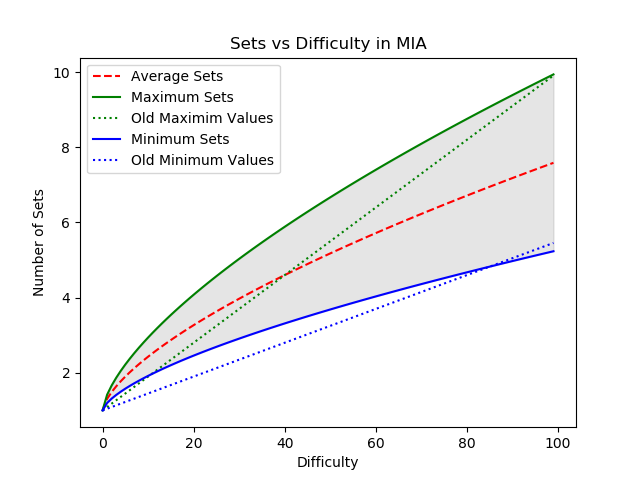
\includegraphics[width=0.5\textwidth]{images/Svd.png}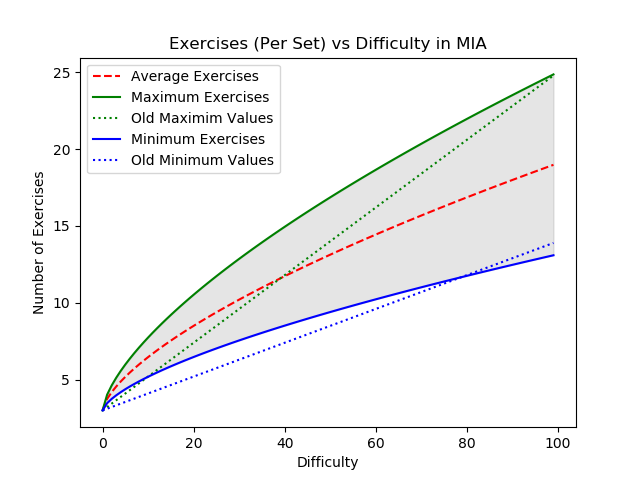
\includegraphics[width=0.5\textwidth]{images/Evd.png}
	\caption{Number of sets per workout (left) and number of exercises pet set (right) based on the user input difficulty. The small dotted lines represent the original algorithm which was a simple linear increase in difficulty for each parameter. For the above two figures, values of $s_{min}=1.0$, $s_{max} = 10.0$, $e_{min}=3.0$ and $e_{max}=25.0$ were used. The possible values for $S$ and $E$ are shown via the gray shaded areas.} \label{Svd and Evd}
\end{figure}

\subsection{Number of Exercises Per Set}

The number of exercises, denoted $E(e_{min},e_{max},d) \equiv E$ is dependent on three variables. The first two are from the input file which are minNumOfExercises\index{minNumOfExercises}, denoted $e_{min}$ and maxNumOfExercises\index{maxNumOfExercises}, denoted $e_{max}$. The last is the difficulty $d$ which is input by the user upon generation. The maximum number of sets was originally based on a linear increase, however for better optimization of the real world workout difficulties, a custom algorithm was created. The maximum $E_{max}(e_{min},e_{max},d)$ and minimum $E_{min}(e_{min},e_{max},d)$ number of sets per workout are given by
\begin{align}
E_{max}(e_{min},e_{max},d) \equiv E_{max}&= \frac{e_{max}-e_{min}}{10^{4/3}} d^{2/3}+e_{min} \\
E_{min}(e_{min},e_{max},d) \equiv E_{min}&= \frac{e_{max}-1.9 \times e_{min}}{1.9 \times 10^{4/3}} d^{2/3}+e_{min}.
\end{align}
Thus since $E(e_{min},e_{max},d)$ is a random value between these curves, we have
\begin{align}
E_{ave}(e_{min},e_{max},d) \equiv E_{ave} &= \frac{E_{max}+ E_{min}}{2} \\ &= \frac{\left(2.9e_{max}-3.8e_{min}\right)}{3.8 \times 10^{4/3}}d^{2/3}+e_{min} \\
E(e_{min},e_{max},d) &= rand[E_{min}(e_{min},e_{max},d), E_{max}(e_{min},e_{max},d)].
\end{align}
These are shown in Figure \ref{Svd and Evd}. Since this value depends on each set, and there are generally numerous sets per workout, we denote the set within the workout with $i$ such that $1\leq i \leq S$, where $S$ is the total number of sets within a workout. Using this index, $E_i$ becomes
\begin{align}
	E_{i,max}(e_{min},e_{max},d) \equiv E_{max}&= \frac{e_{max}-e_{min}}{10^{4/3}} d^{2/3}+e_{min} \\
	E_{i,min}(e_{min},e_{max},d) \equiv E_{min}&= \frac{e_{max}-1.9 \times e_{min}}{1.9 \times 10^{4/3}} d^{2/3}+e_{min} \\
	E_{i,ave}(e_{min},e_{max},d) \equiv E_{ave} &= \frac{E_{max}+ E_{min}}{2} \\ &= \frac{\left(2.9e_{max}-3.8e_{min}\right)}{3.8 \times 10^{4/3}}d^{2/3}+e_{min} \\
	E_i(e_{min},e_{max},d) &= rand[E_{i,min}(e_{min},e_{max},d), E_{i,max}(e_{min},e_{max},d)].
\end{align}
Following this, the average number of exercises done for a given workout would be
\begin{align}
	E_{W} = \frac{1}{S}\sum_{i=1}^{S}E_i.
\end{align}

\begin{figure}[h]
	\centering
	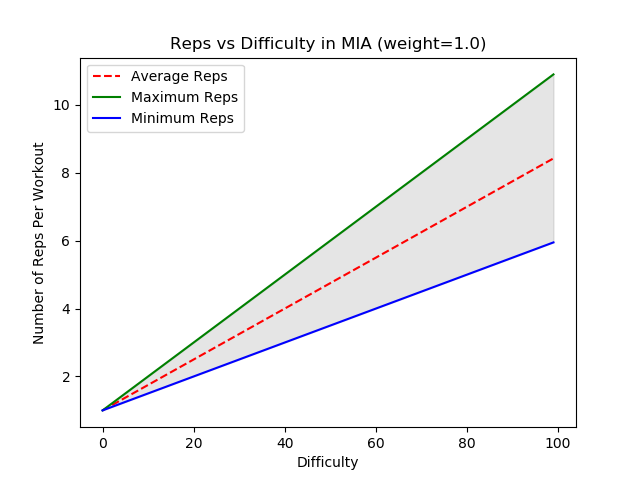
\includegraphics[width=0.5\textwidth]{images/Rvd1.png}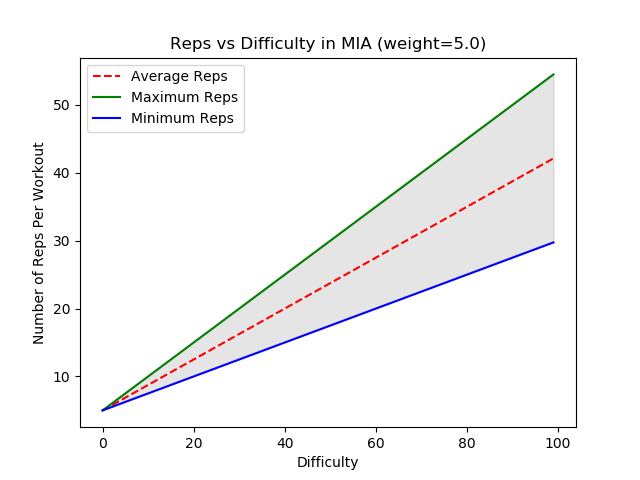
\includegraphics[width=0.5\textwidth]{images/Rvd5.png}
	\caption{Number of reps per exercise. On the right, we have $R(0.1,d,1)$ and on the left, $R(0.1,d,5)$. The possible values for $R$ are shown via the gray shaded area.} \label{Rvd}
\end{figure}


\subsection{Number of Reps Per Exercise}

The number of reps, denoted $R(t,d,w) \equiv R$ is dependent on three variables. The first is toughness $t$ which is gathered from the input file or defaults to 0.1. The second is difficulty $d$ which is input by the user upon generation. Lastly, the weight $w$ of a given exercise is needed to provide the total reps that are output. The reps are determined by a linear trend given by
\begin{align}
	R_{max}(t,d,w) &= tdw+w \\
	R_{min}(t,d,w) &= \frac{tdw}{2}+w \\
	R_{ave}(t,d,w) &= \frac{R_{max}+R_{min}}{2} = \frac{3tdw}{4}+w \\
	R(t,d,w) &= rand[R{min}(t,d,w),R_{max}(t,d,w)].
\end{align}
These are shown in Figure \ref{Rvd}. Since this value depends on each exercise, and there are generally numerous exercises per set, we denote the exercises within the set by an index $j$ such that $1 \leq j \leq E_i$, where $E_j$ is the total number of exercises within the given set $i$. Using this index, $R$ becomes
\begin{align}
	R_{j,max}(t,d,w_j) &= tdw_j+w_j \\
	R_{j,min}(t,d,w_j) &= \frac{tdw_j}{2}+w_j \\
	R_{j,ave}(t,d,w_j) &= \frac{R_{max}+R_{min}}{2} = \frac{3tdw_j}{4}+w_j \\
	R_j(t,d,w_j) &= rand[R_{j,min}(t,d,w_j),R_{j,max}(t,d,w_j)].
\end{align}
Following this, the average number of normalized reps done per set would be
\begin{align}
	R_{i,ave} = \frac{1}{E_i}\sum_{j=1}^{E_i}\frac{R_j}{w_j}.
\end{align}
Then, the average number of reps (normalized by the weights) done per workout would be given by
\begin{align}
	R_{W} = \frac{1}{S}\sum_{i=1}^{S}\frac{1}{E_i}\sum_{j=1}^{E_i}\frac{R_j}{w_j}
\end{align}

\section{Real World Difficulties} 

Due to the way that we set up the weighted system for each exercise, we can easily determine how difficult, denoted $D$ a workout is in reality based upon the generation. First, a workout is directly proportional to the number of sets it contains and thus $D \propto S$. Similarly, the difficulty of each set is proportional to the number of exercises are contained within each set and thus we use $D \propto E_{W}$. Lastly, the difficulty of each exercise is proportional to the number of normalized reps, and thus $D \propto E_{W}$. By combining all of these components we get
\begin{align}
	D \equiv S E_{W} R_{W} = S \left(\frac{1}{S}\sum_{i=1}^{S}E_i \right)\frac{1}{S}\sum_{i=1}^{S}\frac{1}{E_i}\sum_{j=1}^{E_i}\frac{R_j}{w_j}.
\end{align}

To demonstrate the possible values that can be output by $D$ we can examine the maximum and minimum values. The maximum value would be when $S$, $E$, and $R$ are at their maximums. Thus, we have
\begin{align}
	D_{max} &= S_{max} \left(\frac{1}{S_{max}}\sum_{i=1}^{S_{max}}E_{i,max} \right)\frac{1}{S_{max}}\sum_{i=1}^{S_{max}}\frac{1}{E_{i,max}}\sum_{j=1}^{E_{i,max}}\frac{R_{j,max}}{w_j}.
\end{align}
Since each $E_{i,max}$ and $R_{j,max}/w_j$ are the same for all $i,j$ respectively, then we can simplify this to
\begin{align}
	D_{max} &= S_{max} \left(\frac{1}{S_{max}}S_{max}E_{max} \right)\frac{1}{S_{max}}S_{max}\frac{1}{E_{max}}E_{max}\frac{R_{max}}{w} \\
	&= S_{max} E_{max} \frac{R_{j,max}}{w_j}.
\end{align}
Similarly, the minimum value is 
\begin{align}
	D_{min} = S_{min} E_{min} \frac{R_{j,min}}{w_j},
\end{align}
where $R_{j,min}/w_j$ represents the normalized reps for each exercise in both of the above two cases. The possible values of $D$ then lie between these two curves and can be seen in figure \ref{Dvd}.

\begin{figure}[h]
	\centering
	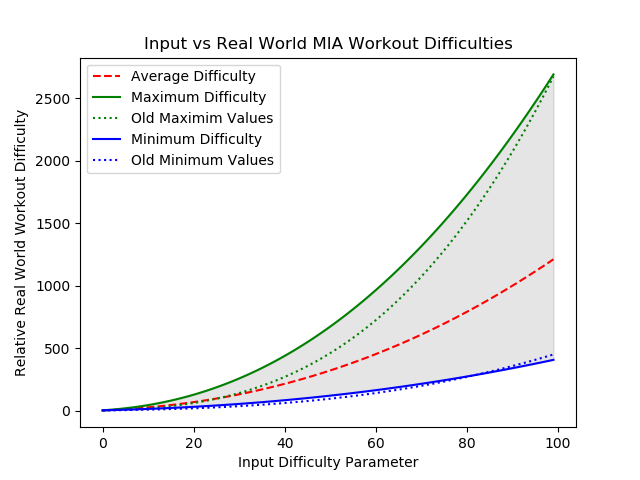
\includegraphics[width=0.5\textwidth]{images/Dvd.png}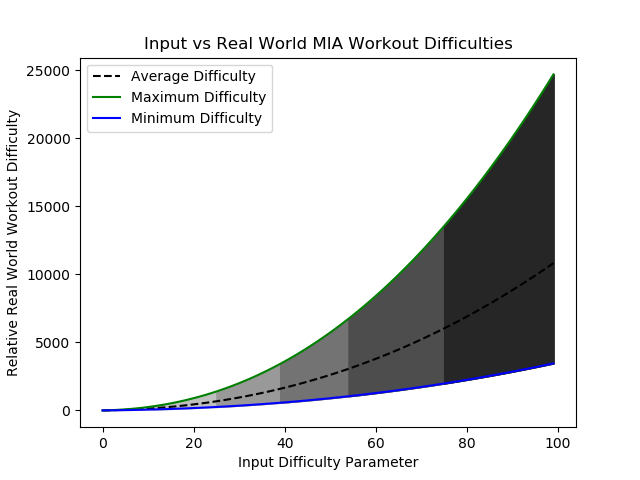
\includegraphics[width=0.5\textwidth]{images/Dvdc.png}
	\caption{The real world difficulties $D$ output by the MIA workout generation program versus the input difficulty parameter (LEFT). The possible values for $D$ are shown via the gray shaded area. The old min/max values represent $D$ based on the old $S$ and $E$ values (see figure \ref{Svd and Evd}). On the right is the same plot only depicting the difficulty ranges. The ranges run from very easy (light gray), to very hard (dark gray).} \label{Dvd}
\end{figure}

The real world difficulty $D$ has an exponential increase. This is desired for a specific reason. As improvements are made, meaning as ones physique and ability to perform improves, a greater challenge is needed. Similarly, there is a much larger variance in the real world difficulty $D$ increases with respect to the input difficulty $d$. This is because as workout intensities increase, there is a desire to keep the body both guessing and not straining too often. Therefore, by increasing the variability of a workout, there is a greater effectiveness and an improved 'rest' or 'slow' period between intensive workouts. 

\section{Notes on Appropriate MIA Parameters For Usage}

Based on the way MIA generates workouts (as described in the above sections), there are a few things to keep in mind when determining the proper settings. First, if a maxNumberOfExercises value of 'inf' is used, then the real world difficulty output will be proportional to the number of exercises defined in the input file. Therefore, if one places a thousand different workouts in this file, each difficulty will be drastically more intense than if there were only 25. Thus, it is important to experiment with this value and adjust accordingly based on the number of defined exercises you have in the input file.

 



\chapter{World of Warcraft (WoW) Features in MIA} \label{WoW}
\pagestyle{fancy}

\section{WoW Fishbot} \label{WoWFishbot}

\begin{note}
	This fishbot was made for educational purposes only! Do not use this in the game or you may be banned as it violates the license agreement! As of World of Warcraft (WoW) version 7.2, this fishbot is fully functional.
\end{note}

The World of Warcraft (WoW) fishbot implementation within MIA was created solely for educational purposes. This fishbot violates the terms of use of WoW and should only be used at your own risk. The fishbot is designed to simulate fishing for ones character in WoW. 

\subsection{Setup and Configuration}

Before running the fishbot, there are a few things that need to be properly configured, otherwise the bot will either not work or not work efficiently. First, one must disable the hardware cursor in the system settings. This can be done by pressing escape, system, advanced, then setting hardware cursor to disable (see figure \ref{hardwar cursor}). Be sure to click apply before closing out of the settings.

\begin{lstlisting}
ESC > System > Advanced > Hardware Cursor > DISABLE > Apply
\end{lstlisting}

\begin{figure}[h]
	\centering
	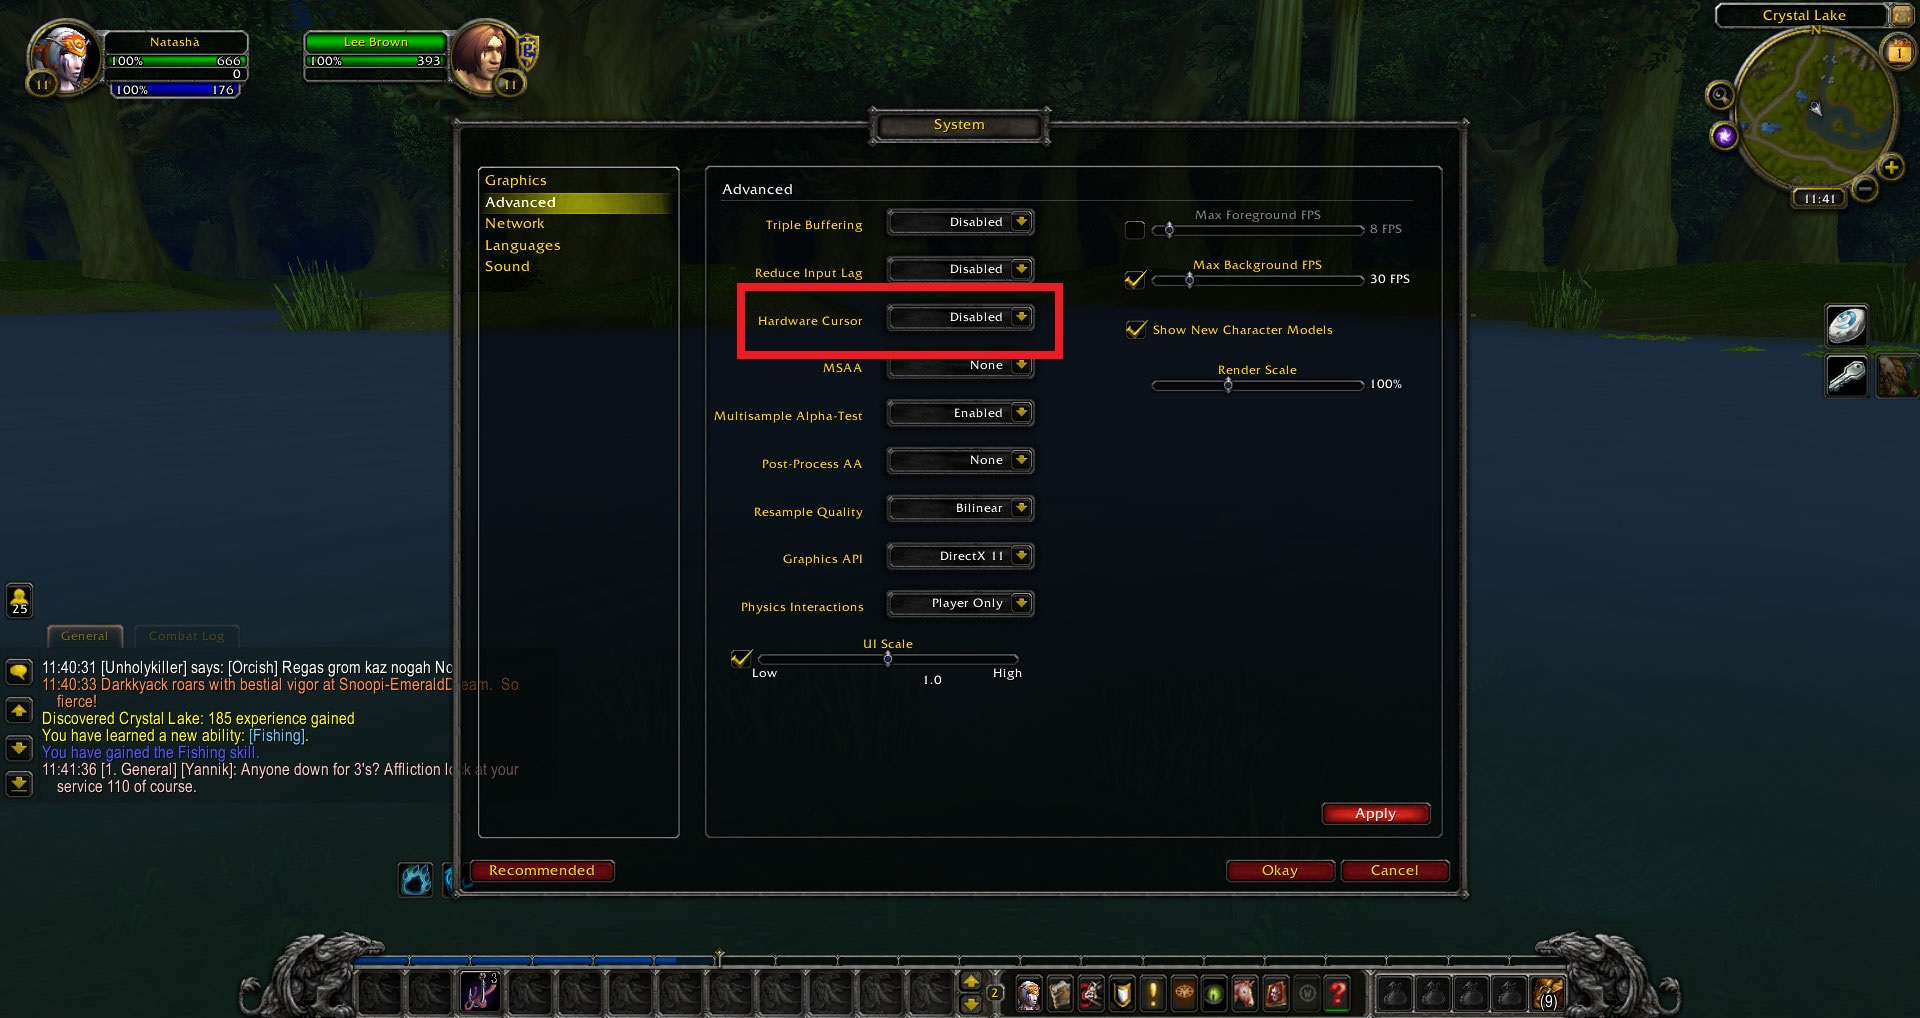
\includegraphics[width=0.9\textwidth]{images/WoWScrnShot_040118_234154.jpg}
	\caption{Visual representation of the location of the option for disabling the hardware cursor. In order for the WoW fishbot to work, this option must be disabled.} \label{hardwar cursor}
\end{figure}

After disabling the hardware cursor, the coordinates for cast locations need to be set. It is recommended that the user zoom into first person when using the fishbot though this is not required for functionality. First, place the cast button on the action bar (see figure \ref{cast bar}). By default, the fishbot uses button 3 for cast, but upon running the fishbot the user will be prompted to change the settings. Similarly, a lure can be added to the bar, which by default is placed in action bar slot 8. A lure is optional and the fishbot program will ask if one is being used upon runtime.

\begin{figure}[h]
	\centering
	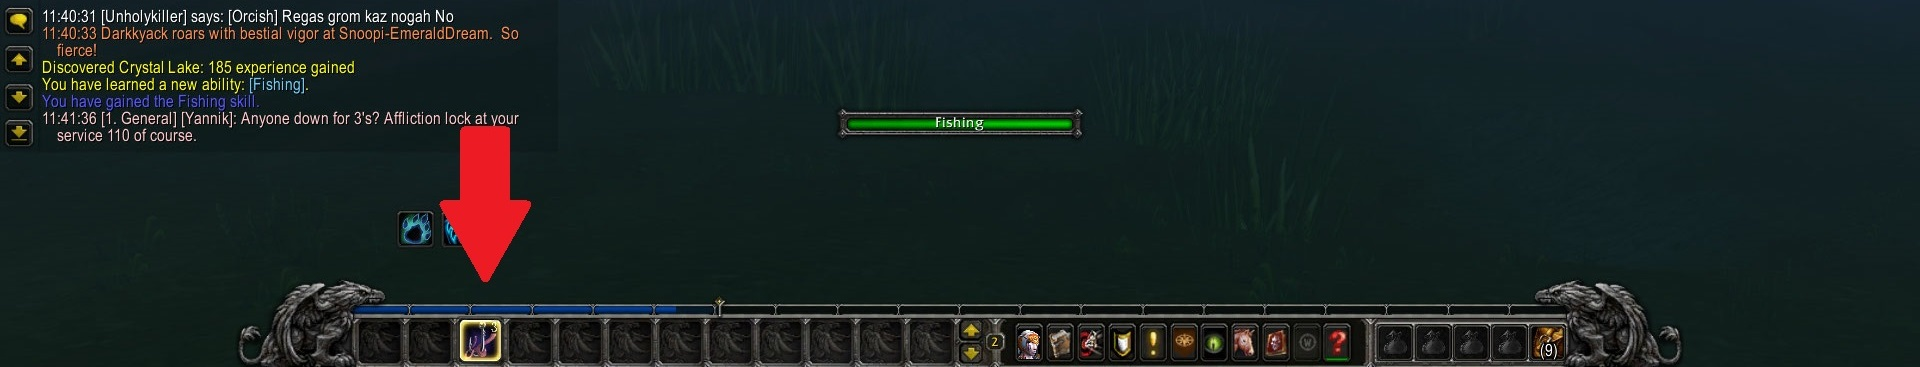
\includegraphics[width=0.9\textwidth]{images/WoWScrnShot_040118_234212.jpg}
	\caption{Visual representation of the location of the cast option on the action bar.} \label{cast bar}
\end{figure}

The WoW-specific configuration variables are now contained in a separate configuration file named \texttt{WoWConfig.MIA}. This file includes several settings related to WoW apps and tools within MIA, including variables for the fishbot implementation. Unlike the previous defaults embedded in MIAC (in prior MIA versions), these values are centralized here for easier customization. Some of the fishbot-related variables, along with their current defaults, are shown below:

\begin{lstlisting}[style=pythonstyle]
# Variables relating to the fishbot implementation inside MIA.
WoWFishBotStartX=791
WoWFishBotStartY=443
WoWFishBotEndX=1082
WoWFishBotEndY=581
\end{lstlisting}

\begin{figure}[h]
	\centering
	
\includegraphics[width=0.8\textwidth]{images/WoWScrnShot_040118_234212b.jpg}
	\caption{The red square represents the region in which the casted bobber lands. The two points labeled A and B are positions that one would want to set as the proper coordinates in the configuration file.} \label{fishbot square}
\end{figure}

These values, \texttt{WoWFishBotStartX, WoWFishBotStartY, WoWFishBotEndX, WoWFishBotEndY}, define the area that the fishbot will search for the fish bobber within. The first two parameters, \texttt{WoWFishBotStartX, WoWFishBotStartY} define the coordinates of the point A in figure \ref{fishbot square}. The second two parameters, \texttt{WoWFishBotEndX, WoWFishBotEndY} define the coordinates of the point B in figure \ref{fishbot square}. The MIA fishbot will search this area for the bobber during operation. The best method to determine the proper coordinates to use is to spam the cast option and observe the area that the bobber lands. The suggested coordinates for A and B are near where they are located in figure \ref{fishbot square}, however any coordinates can be used. To determine the proper coordinates, one can use the \texttt{find mouse} command in MIA which will determine the coordinates at the location of ones cursor.

After these parameters are set, the fishbot can be run in MIA by using the \texttt{fishbot} command. There are a few other variables and parameters that can be set by the user but the others are optional. These other optional parameters that are contained in the configuration file are as follows.

\begin{lstlisting}[style=pythonstyle]
# Variables relating to the fishbot implementation inside MIA.
WoWFishBotIncrement=40
WoWFishBotNumOfCasts=10000
WoWFishBotDelay=10000
\end{lstlisting}

First, the \texttt{WoWFishBotIncrement} variable defines the step size that the MIA program will search for the bobber by. This can be seen in figure \label{fishbot increments}. A smaller step size will cause the fishbot to find the bobber slower but more accurate, whereas a faster step size will cause a faster search but is less accurate. The default value for this is 40, but should be decreased if the bobber is missed by the fishbot. The next parameter, \texttt{WoWFishBotNumOfCasts} is how many times the fishbot will cast before ending it's program. This can be whatever the user desires. 



\begin{figure}[h]
	\centering
	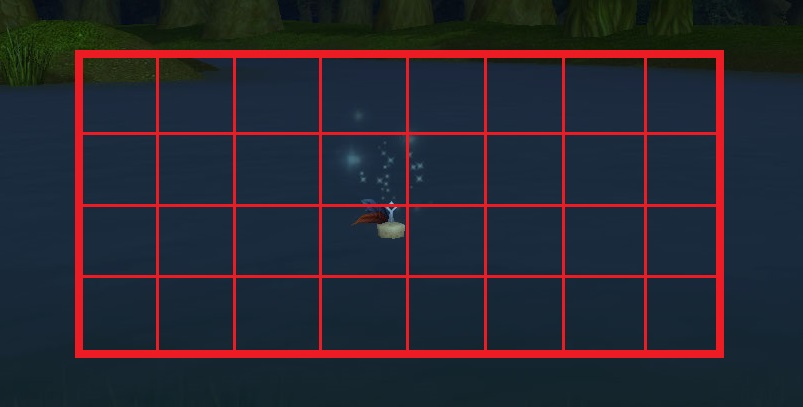
\includegraphics[width=0.8\textwidth]{images/WoWScrnShot_040118_234227b.jpg}
	\caption{The red square similar to that shown in figure \ref{fishbot square} partitioned into squares of size defined by the \texttt{WoWFishBotIncrement} value.} \label{fishbot increments}
\end{figure}

\begin{figure}[h]
	\centering
	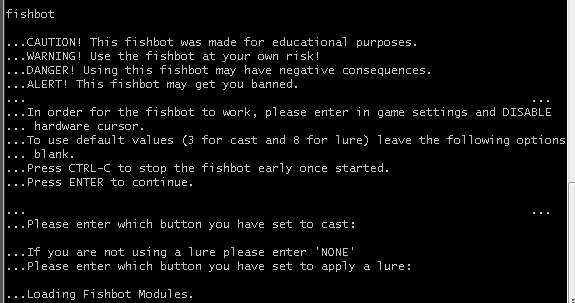
\includegraphics[width=0.7\textwidth]{images/fishbot_MIA.png}
	\caption{A snapshot of the MIA fishbot upon runtime. As of MIA version 0.041.} \label{fishbot terminal}
\end{figure}

The last parameter, \texttt{WoWFishBotDelay} is what defines how fish are caught. The MIA fishbot catches fish by chance. There is a plan to improve the method to catch fish by, but for now the program waits a specific number of milliseconds after finding the bobber before clicking it. Thus, there is a certain probability that a fish is caught. By default this value is 10000ms.

To run the fishbot simply use the \texttt{fishbot} command in the MIA terminal. Upon running this command, the fishbot will ask the use to enter the required information (see figure \ref{fishbot terminal})

\section{Mailbox Management} \label{WoWMailbox}

\begin{note}
	This program technically violates the blizzard license agreement and should be used with caution. However, it is no more complicated than an addon. I just happen to know C++ and not lua.
\end{note}

MIA contains some in game mail management for World of Warcraft (WoW) in order to assist in the process of creating in game letters in bulk. In game letters can't be sent between characters and then looted and stored in the character inventories. In some cases, such as role playing (RP) or guild recruitment, these letters may be desired by bulk. The process of creating these letters consists of entering in a letter recipient, subject, the contents of the letter, and then hitting a send button (see figure \ref{wow mailbox send}). After sending these letters, however many times it is done, they then need to be looted on the character that they were sent to. This consists of opening up the mailbox, clicking on the letter received, acquiring the physical copy by looting it from the opened letter, then deleting the letter to clean up the mailbox (see figure \ref{wow mailbox receive}). MIA is designed to automate this entire process.

\subsection{Sending Duplicates of a Letter}

As described above briefly, MIA has the capability of automating the sending of duplicate letters to a recipient in WoW. To do this, there are a few settings that need to be configured on the user end to ensure proper functionality. There are two variables contained in the configuration file that are used in conjunction with the \texttt{wow dup letter} function in MIA. These are listed below.

\begin{lstlisting}[style=pythonstyle]
# WoW related variables.
WoWMailboxSendLetterLocationX=279
WoWMailboxSendLetterLocationY=647
\end{lstlisting}

By default, these values are set for the environment that was used when originally programmed into MIA. Both of these variables are used to represent the location of the send button shown in figure \ref{wow mailbox send}. The first, \texttt{WoWMailboxSendLetterLocationX} represents the x coordinate and the latter \texttt{WoWMailboxSendLetterLocationY} represents the y coordinate. Both of these values can be found by using the \texttt{find mouse} function in MIA. 

\begin{figure}[h]
	\centering
	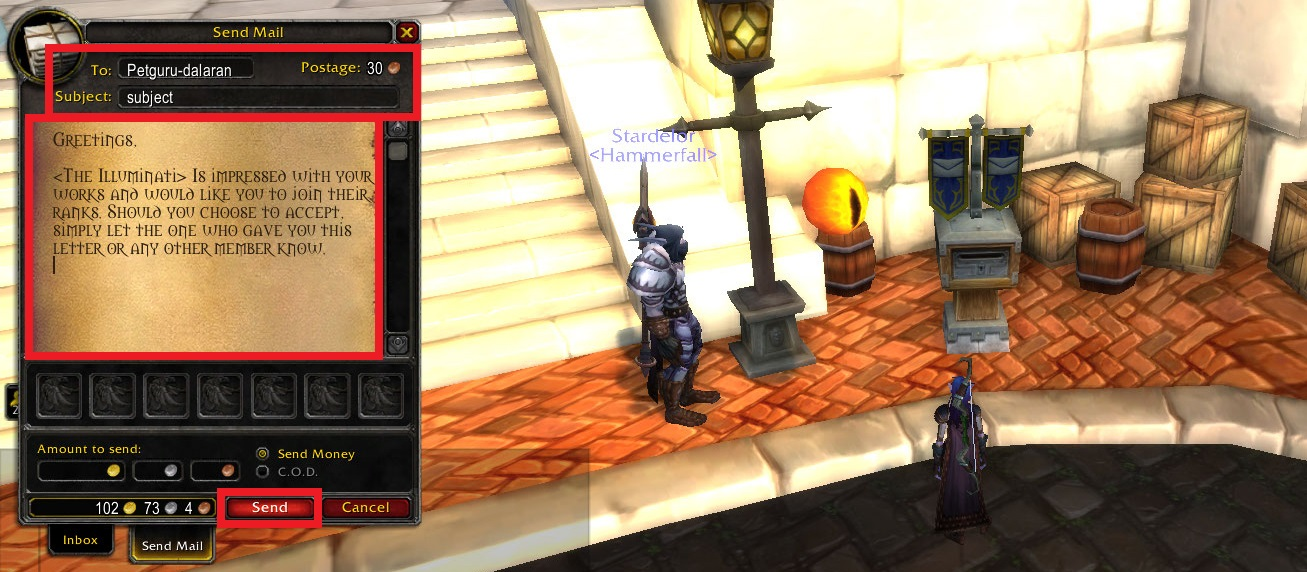
\includegraphics[width=0.9\textwidth]{images/WoWScrnShot_040518_181350b.jpg}
	\caption{A screen shot of the WoW in game outgoing mailbox menu. The mail management within MIA utilizes the fields indicated by red squares in this menu. The red box around the send button represents the \texttt{WoWMailboxSendLetterLocation} location.} \label{wow mailbox send}
\end{figure}

Once the proper coordinates are set, one can automate this process of sending a duplicate letter by using the \texttt{wow dup letter} command in the MIA terminal. The \texttt{wow dup letter} has a few limitations when used. First, the recipient of the letter can only contain normal characters such as a, e, o, etc. The recipient cannot contain special characters such as \"{a}, \'{e}, \~{o}, etc. However, the contents of the message that will be sent can contain special characters. The desired message contents should be copied to the clipboard before running the \texttt{wow dup letter} command. Upon running the command, the terminal will prompt the user to do so as well. The subject field will automatically be filled in with "subject."

\begin{figure}[h]
	\centering
	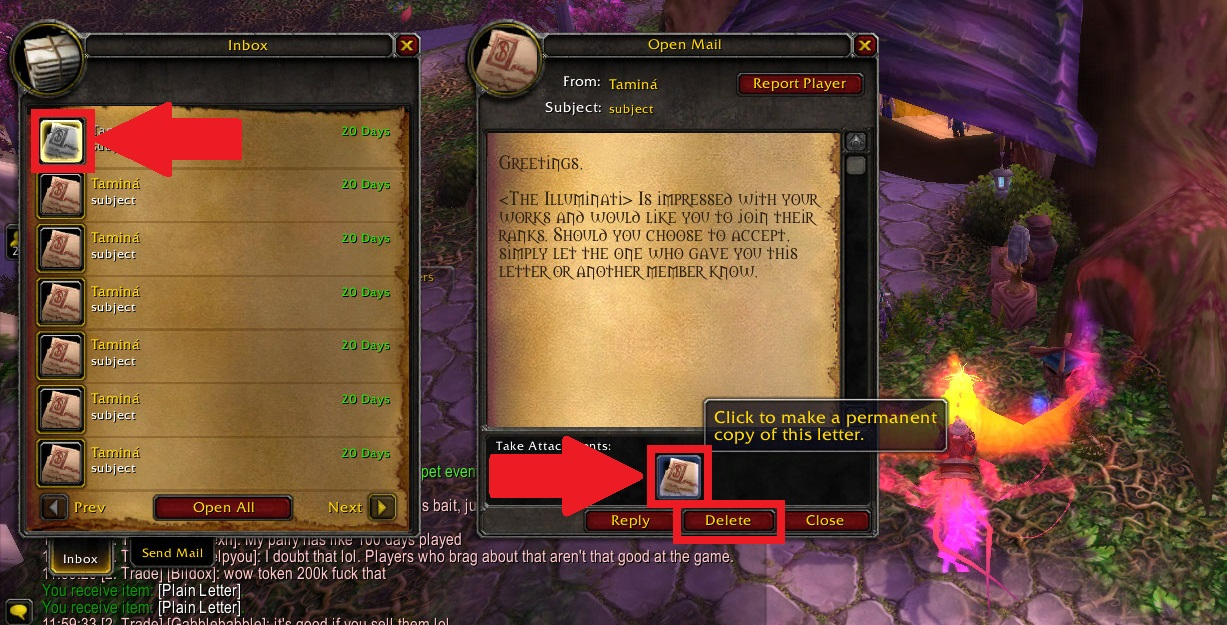
\includegraphics[width=0.9\textwidth]{images/WoWScrnShot_040518_115947b.jpg}
	\caption{A screen shot of the WoW in game incoming mailbox menu. The mail management within MIA utilizes the fields indicated by red squares in this menu. The left arrow indicates the \texttt{WoWMailboxFirstLetterLocation} position. The right arrow indicates the \texttt{WoWMailboxLootLetterLocation} position. The square around the delete button represents the \texttt{WoWMailboxDeleteLetterLocation} location.} \label{wow mailbox receive}
\end{figure}

\subsection{Unloading Duplicated letters}

MIA contains a command \texttt{wow unload} which is designed to be used in conjunction with the \texttt{wow dup letter} command. This command will loot the letters from the incoming mailbox that are sent using the \texttt{wow dup letter} command. In order to use this command properly, there are six different variables within the configuration file that need to be determined for the users environment. These variables are below.

\begin{lstlisting}[style=pythonstyle]
# WoW related variables.
WoWMailboxFirstLetterLocationX=55
WoWMailboxFirstLetterLocationY=265
WoWMailboxLootLetterLocationX=675
WoWMailboxLootLetterLocationY=600
WoWMailboxDeleteLetterLocationX=700
WoWMailboxDeleteLetterLocationY=650
\end{lstlisting}

By default, these variables are set to values that were specific to the programmers environment. The variables need to be set based off of three different coorindates. The first, \texttt{WoWMailboxFirstLetterLocation} corresponds to the location of the first letter in the inbox of the user (see figure \ref{wow mailbox receive}). The second, \texttt{WoWMailboxLootLetterLocation} corresponds to the location of the letter to loot from the user inbox (see figure \ref{wow mailbox receive}). The last, \texttt{WoWMailboxDeleteLetterLocation} represents the locations of the delete button on a letter in the WoW inbox (see figure \ref{wow mailbox receive}).  For all three coordinates, there is an x and y value (represented by the variables in the configuration file) which can be determined through MIA by using the \texttt{find mouse} command.
\chapter{Coding Standards} \label{ch:coding-standards}
\pagestyle{fancy}

\textbf{IMPORTANT:} These coding standards are still being developed and not finished or finalized. They can safely be followed, but some parts may change, or additions will be made in the future.

\section{Overview}

As of MIA version 2\footnote{Note: Although the coding standards are adopted in version 2, not all of the code yet conforms to this standard. Much of the old code which was migrated over still needs improvements and fixes in order to fit these standards.}, a set of coding standards has been adopted by this project. To maintain consistency, readability, and maintainability across the project, a unified coding standard for all C++, CMake, and Bash code is used. This section outlines the conventions and best practices to be followed by all current and future contributors. Adhering to these guidelines helps reduce bugs, ease code reviews, and improve collaboration if MIA ever became a multi-developer environment.

Since this project was (and still is at the time of writing this) solely for personal edification, learning, and experimentation, its primary purpose has been to explore new tools, techniques, and patterns across C++, CMake, and Bash. However, it also serves as a practical demonstration of my coding style and development practices - much like a portfolio, though firmly within the realm of hobby code. As such, while the codebase may not meet production-level rigor in every detail, this coding standards documentation exists to highlight the conventions I choose to follow, the rationale behind them, and how they reflect what I believe to be a synthesis of the best practices across the diverse landscape of existing standards. This includes adapting principles from well-known style guides while also incorporating personal preferences that I’ve found to improve clarity, maintainability, and efficiency through hands-on experience.

\section{C++ Coding Standards}

\subsection{Formatting and Style}
\begin{itemize}\itemsep0em
    \item \textbf{Indentation}: Use \texttt{spaces} with a width of \texttt{4} spaces.
    \item \textbf{Line length}: Limit lines to \texttt{120} to \texttt{140} characters. Traditionally, less characters are used. However, with newer computers and displays, this rarely makes sense. With a \texttt{120} to \texttt{140} width, most modern-sized computer displays can display 2-3 columns/files of code at a time wth an additional file-browser window. The range in values comes from a standput of developer discretion. Often times, a hard cap at a set line length can produce some fairly unappealing code and less readable, where the, range allows the developer to use discretion based on the code itself. 
    \item \textbf{Brace placement}: \texttt{Allman}. Although the original MIA project was in K\&R format, I've chosen to move to \texttt{Allman} as of version 2. The benefits of Allman include the following:    
    \begin{itemize}\itemsep0em
        \item Aligned Blocks: With Allman, readability is often enhanced because you do not have to visually search the end of variable-length lines for brackets or rely on tabs. Allman can help reduce cognitive load when scanning code. All brackets are at the start of the line and aligned with the ending bracket. 
        \item Clearly Separated Blocks: This style makes each block of code more clearly separated.
        \item Commenting: The initial bracket of a code block can serve as a perfect spot for a brief comment related to the block itself. 
    \end{itemize}
    \item \textbf{Naming conventions}:
    \begin{itemize}\itemsep0em
        \item Classes and structs: \texttt{PascalCase}
        \item Enums and typedefs: \texttt{PascalCase}
        \item Functions and methods: \texttt{camelCase}
        \item Variables: \texttt{camelCase}
        \item Constants: \texttt{ALL\_CAPS} 
    \end{itemize}
\end{itemize}

\subsection{Code Organization and Practices}
\begin{itemize}\itemsep0em
    \item Header files should include include guards or \texttt{\#pragma once}.
    \item Prefer smart pointers over raw pointers where ownership is involved. Smart pointers such as \texttt{std::unique\_ptr} and \texttt{std::shared\_ptr} manage memory automatically and help prevent common issues like memory leaks, dangling pointers, and double deletions. They make ownership semantics explicit and integrate with RAII (Resource Acquisition Is Initialization), ensuring that resources are properly released when no longer needed. Raw pointers can still be used for non-owning references, but ownership should be clearly represented through smart pointers to improve code safety and maintainability.    
    \item Avoid using \texttt{using namespace std;} in headers. Placing \texttt{using namespace} directives in headers pollutes the global namespace for any file that includes that header, potentially causing name collisions and ambiguous references. This can lead to subtle and hard-to-debug errors, especially in large codebases or when integrating with third-party libraries. Instead, fully qualify names (i.e., \texttt{std::vector}) in headers to keep dependencies explicit and avoid unintended side effects.
    \item Separate declaration and implementation: use headers (\texttt{.hpp}) for interfaces and source files (\texttt{.cpp}) for implementation.
    \item Prefer forward declarations over includes in headers when only a pointer or reference to a type is needed. Only include full headers when access to the complete type is required.
    \item Where applicable, default fallback values (i.e., 0, "", false) may be returned in lieu of exceptions for non-critical failures, provided this behavior is explicitly documented. This includes all get*() functions for configuration access.
    \item Exceptions should be used only for unrecoverable errors or contract violations, and custom exceptions (i.e., MIAException) should encapsulate error context where possible.
    \item Use Resource acquisition is initialization (RAII) for resource management.
    \item Use const correctness to express immutability.
    \item Document all public interfaces with Doxygen-style comments.
\end{itemize}



\subsection{Virtual Classes, Abstractions, and PIMPL}

Object-oriented abstractions such as virtual classes and the PIMPL (Pointer to Implementation) idiom are powerful tools but must be used judiciously to avoid unnecessary complexity and indirection. Code should prioritize readability and simplicity over overengineering. Clear, straightforward implementations are easier to maintain, debug, and extend than overly abstract or generalized solutions. Avoid premature optimization or architectural complexity unless justified by concrete requirements. The goal is to make the intent and behavior of the code immediately understandable to other developers. When in doubt, favor code that communicates clearly over code that attempts to be overly clever or flexible without a proven need.

\subsubsection*{Virtual Classes and Abstract Interfaces}

Abstract classes (i.e., classes with pure virtual functions) should be used to define clean, minimal interfaces that enable polymorphism and decouple high-level logic from specific implementations. These interfaces are particularly appropriate in the following cases:
\begin{itemize}\itemsep0em
    \item Multiple interchangeable implementations are required.
    \item Code must be testable via mocks or stubs.
    \item A plugin or extensibility mechanism is being designed.
\end{itemize}
Avoid over-engineering by introducing interfaces prematurely. When there is no clear need for polymorphism, prefer concrete classes for simplicity and clarity. Overall, free-functions are preferred where applicable.

\subsubsection*{PIMPL Idiom}

The PIMPL idiom may be used to encapsulate implementation details and reduce compilation dependencies, particularly for public interfaces that are expected to remain stable while their internals may change. Its use must be justified by the need to isolate dependencies, improve build performance, or enforce ABI stability. The PIMPL (Pointer to Implementation) idiom is used to:
\begin{itemize}\itemsep0em
    \item Hide private data members and internal implementation details.
    \item Reduce build dependencies and improve compilation times.
    \item Achieve binary interface stability across library versions.
\end{itemize}

PIMPL should only be used when these benefits are specifically needed. It introduces runtime indirection and heap allocation, which may be unnecessary in simpler or performance-sensitive components.
\begin{lstlisting}[style=cppstyle]
/**
 * @brief A class demonstrating the PIMPL idiom for encapsulation.
 */
class MyClass 
{
public:
    /**
     * @brief Constructs a MyClass instance.
     */
    MyClass();
    
    /**
     * @brief Destroys the MyClass instance, freeing resources.
     */
    ~MyClass();
private:
    class Data; ///< Forward declaration of implementation details.
    std::unique_ptr<Data> data; ///< Pointer to implementation.
\end{lstlisting}

\paragraph{Usage Guidelines}

\begin{itemize}\itemsep0em
    \item Use virtual functions only where dynamic behavior is explicitly required.
    \item Keep interfaces small, focused, and consistent.
    \item Use PIMPL for library boundaries or complex internals where ABI stability or encapsulation justifies the added indirection.
    \item Avoid using PIMPL as a default or substitute for proper modular design.
\end{itemize}

By adhering to these principles, the code remains both flexible and maintainable without incurring the overhead of unnecessary abstraction.



\subsection{Attributes, Specifiers, and Member Annotation Standards}

\subsubsection*{C++ Attribute Specifiers}

C++ standard attributes such as \texttt{\textbf{[[deprecated]]}}, \texttt{\textbf{[[maybe\_unused]]}}, and others should be used appropriately to enhance clarity, compiler diagnostics, and maintainability.
\begin{itemize}\itemsep0em
  \item \textbf{\texttt{[[deprecated]]}} \\
  Use to mark deprecated interfaces explicitly. Always include an explanatory message:
  \begin{lstlisting}[style=cppstyle]
[[deprecated("Use newMethod() instead")]]
void oldMethod();
  \end{lstlisting}

  \item \textbf{\texttt{[[maybe\_unused]]}} \\
  Apply to functions or variables that may be unused in some contexts (i.e., for debugging or optional features):
  \begin{lstlisting}[style=cppstyle]
[[maybe_unused]]
void dumpConfigMap(std::ostream& os = std::cout) const;
  \end{lstlisting}

  \item \textbf{\texttt{[[nodiscard]]}} \\
  Use for return values where the result must be used by the caller (i.e., for error codes or ownership types).
\end{itemize}
Use attribute specifiers only when their intended behavior is part of the API contract or serves a specific, useful purpose. Avoid excessive or speculative use.

\subsubsection*{\texttt{override} and \texttt{final} Usage}

All overridden virtual methods must be explicitly marked with \texttt{override}. Do \textbf{not} use the \texttt{virtual} keyword on the overriding declaration.
\begin{itemize}\itemsep0em
  \item Correct:
  \begin{lstlisting}[style=cppstyle]
void onStart() override;
  \end{lstlisting}
  \item Incorrect:
  \begin{lstlisting}[style=cppstyle]
virtual void onStart() override;
  \end{lstlisting}
\end{itemize}
Use \texttt{final} on classes or methods where further subclassing or overriding is explicitly disallowed:
\begin{lstlisting}[style=cppstyle]
class Logger final { ... };
void onShutdown() final;
\end{lstlisting}


\subsection{Comments and Documentation}

All code elements including classes, namespaces, methods, typedefs, variables, and files must have Doxygen comments. These comments should primarily be placed in header files to serve as the main documentation source. For methods not declared in headers but implemented in \texttt{.cpp} files, corresponding Doxygen comments should be added in the implementation files. In-code comments must be sufficiently informative to allow any developer to understand the purpose, usage, and modification requirements of the code without needing to consult external documentation. This includes describing the intent of classes and methods, explaining parameters and return values, and clarifying design decisions where applicable.

In \texttt{.cpp} implementation files, comments should be added at the developer’s discretion but are ideally included:
\begin{itemize}\itemsep0em
    \item Before blocks of code that perform distinct tasks,
    \item When specific literal values or “magic numbers” are used for particular reasons,
    \item Where behavior might not be immediately clear from the code itself,
    \item To highlight important side-effects or assumptions.
\end{itemize}
For ease of navigation and maintenance, closing braces of namespaces, classes, and long code blocks should be followed by simple trailing comments indicating their scope, for example:
\begin{lstlisting}[style=cppstyle]
} // namespace myNamespace
\end{lstlisting}
This convention helps match braces quickly without excessive scrolling.

\subsubsection*{Additional guidelines}
\begin{itemize}\itemsep0em
    \item Avoid redundant comments that restate obvious code.
    \item Use complete sentences, present tense, punctuation, and consistent phrasing for clarity.
    \item Use consistent terminology and formatting in all comments.
    \item Prefer clarity and brevity over verbosity.
    \item Update comments promptly alongside code changes to keep them accurate.
    \item All functions that may throw exceptions must document them using @throws. 
\end{itemize}

\subsubsection*{Example Doxygen comments}

For multi-line comments, use the \texttt{/** .. */} comment block.
\begin{lstlisting}[style=cppstyle]
/**
 * @brief Represents a configurable widget.
 * This class manages widget configuration and state.
 * @param config[Config] - Configuration settings for the widget.
 * @return Widget instance initialized with given config.
 */
class Widget 
{
public:
    /**
     * @brief Initializes the widget with given settings.
     * @param settings[Config] - The configuration to apply.
     */
    void initialize(const Config& settings);
};
\end{lstlisting}
For single-line comments that document member variables, use \texttt{///} directly above the definition. These comments should be clear, concise, and written in full sentences when appropriate.
\begin{lstlisting}[style=cppstyle]
/// The name of the configuration file for this object.
std::string configFileName;
\end{lstlisting}
\textbf{Guidelines:}
\begin{itemize}\itemsep0em
    \item Use \texttt{///} rather than \texttt{//} for documentation intended to be parsed by tools like Doxygen.
    \item Comments must describe the purpose or semantics of the variable, not its type or structure (which should be clear from the code).
    \item Maintain grammatical consistency and use proper punctuation.
\end{itemize}
Each enumeration should be preceded by a Doxygen-style comment block explaining its purpose. Individual enum values must use \texttt{///<} inline comments to document their meaning. This ensures that documentation tools capture the purpose of each constant clearly, and that readers can understand the intent without leaving the context of the declaration.
\begin{lstlisting}[style=cppstyle]
/**
 * These are the various actions which the sequencer supports.
 */
enum SequenceActionType
{
    UNKNOWN,     ///< Unknown action - do nothing.
    TYPE,        ///< This will type a sequence of characters.
    SLEEP,       ///< This will wait/pause some time.
    DELAY,       ///< This is the time to wait between each action.
    MOVEMOUSE,   ///< This will move the mouse to a specific coordinate.
    CLICK        ///< This will perform a click with the mouse.
};
\end{lstlisting}
\textbf{Guideline:} Always use \texttt{///<} on the same line as the enum value, not on a new line above. Comments should be concise, use present tense, and describe the runtime behavior.


\subsubsection*{Line Comments in Implementation Files}

Use \texttt{//} for brief, inline, or explanatory comments within function implementations. These should clarify logic, document assumptions, or highlight non-obvious decisions.
\begin{lstlisting}[style=cppstyle]
// Apply default configuration values if not explicitly set
if (!settings.hasTimeout()) 
{
    settings.setTimeout(DEFAULT_TIMEOUT); // DEFAULT_TIMEOUT defined in config.h
}
\end{lstlisting}
\begin{lstlisting}[style=cppstyle]
// Bad: Sets timeout to default
settings.setTimeout(DEFAULT_TIMEOUT);

// Good: Use default timeout if none specified in config
settings.setTimeout(DEFAULT_TIMEOUT);
\end{lstlisting}
\textbf{Guidelines:}
\begin{itemize}\itemsep0em
    \item Place standalone comments on their own line above the code they describe.
    \item Use inline comments sparingly and only when the code is not self-explanatory.
    \item Do not restate what the code does—explain why it does it, if not obvious.
    \item Maintain clarity and brevity; comments should add value, not clutter.
\end{itemize}



\subsection{README Files and Higher-Level Documentation}

Each code directory must contain a \texttt{README} file that provides a concise overview of the directory’s purpose. The README should include:
\begin{itemize}\itemsep0em
    \item A brief description of the contents of the directory (key files, subfolders).
    \item The role and relationship of these files or components within the larger project.
    \item Any special instructions or notes relevant to developers navigating or modifying the directory.
\end{itemize}
This ensures quick orientation for developers and aids maintainability across the codebase.

At the project level, comprehensive documentation is maintained in the main MIA manual. This manual offers a high-level overview of:
\begin{itemize}\itemsep0em
    \item The complete set of features and functionality.
    \item Descriptions of libraries and core components.
    \item Available tools and utilities.
    \item Architectural design decisions and workflows.
\end{itemize}
The MIA manual serves as the primary reference for understanding the system holistically and should be kept up-to-date as the project evolves.

Together, directory-level README files and the MIA manual provide layered documentation: granular, file-level guidance paired with broad, conceptual understanding, facilitating both detailed development work and strategic planning.

\subsubsection*{Example README excerpt}

\begin{lstlisting}[style=cppstyle]
# apps Directory Overview

This directory contains the standalone apps for the MIA project. Below is a brief description of each subfolder:
  
- **template/**  
  Contains a fully functional app featuring most of the basic application framework techniques used in developing MIA apps. This is used to both test new features and provide a common template for storing correct usage of the various features.
\end{lstlisting}









\section{CMake Standards}

\subsection{Structure and Conventions}
A clean CMake structure improves build reproducibility and portability. Modern practices enable more maintainable and scalable build definitions. Clear separation of targets and dependencies reduces cross-target pollution.
\begin{itemize}\itemsep0em
    \item Use lowercase CMake commands (i.e., \texttt{add\_executable}, \texttt{target\_link\_libraries}).
    \item Group CMake files logically and modularly using subdirectories and \texttt{add\_subdirectory()}.
    \item Use modern CMake features (i.e., target\_include\_directories, target\_compile\_features).
    \item External dependencies must be managed using \texttt{FetchContent} or \texttt{find\_package}.
    \item Add comments to any blocks of cmake code which function together to perform a particular task. For example:
    \begin{lstlisting}[style=pythonstyle]
# Create the MIATemplate executable.
set(MIATemplate_SRC MIATemplate.cpp MIATemplate_main.cpp )
set(MIATemplate_INC MIATemplate.hpp )
add_executable(MIATemplate ${MIATemplate_SRC} ${MIATemplate_INC} )
target_link_libraries(MIATemplate PRIVATE Core_LIB )
    \end{lstlisting}
\end{itemize}











\section{Bash Scripting Standards}

\subsection{Style and Safety}
\begin{itemize}\itemsep0em
    \item Use \texttt{\#!/bin/bash} (or \texttt{\#!/usr/bin/env bash}) at the top of scripts.
    %\item Always use \texttt{set -euo pipefail} to catch errors early.
    \item Use functions to encapsulate logic (when appropriate) instead of writing top-level scripts.
    %\item Use \texttt{local} keyword inside functions for variable scoping.
    %\item Quote all variable references: \texttt{"\$\{var\}"}.
    %\item Prefer \texttt{\$(...)} over backticks for command substitution.
\end{itemize}

\subsection{Documentation and Naming}
\begin{itemize}\itemsep0em
    \item Start each script with a brief comment block describing its purpose and usage.
    \item Use descriptive function and variable names.
    \item Use comments to clarify non-obvious logic, especially when using subshells or traps.
\end{itemize}











\section{Enforcement and Exceptions}

\begin{itemize}\itemsep0em
    \item Continuous integration pipelines are still in development for this project which will enforce code quality.
    \item If other developers join this project, code reviews will be expected to evaluate adherence to these standards.
\end{itemize}

If a contributor proposes a deviation from these standards for good reason (i.e., performance, cross-platform needs), it must be documented and justified in the merge request. In all other cases, adherence is expected.








\backmatter
%\begin{appendices}

\end{appendices}






%\begin{thebibliography}{99}
	\bibitem{item} 
\end{thebibliography}
\printindex


\end{document}
